% Provenance (never printed): see sources/outline_sources.md (Year 1: grain size and sorting;
% bedforms and sedimentary structures; fluvial, deltaic, shoreline and deep-sea deposits).
% Exercise and problem values in the Book 3 scratch calculator calc/ch21.py; figure data
% from figdata/bachelor-1/grain_size.py. Meander and delta are Book 1's (g5), sediment and
% sedimentary layer Book 1's (g7), beach Book 1's (g9); the loads, settling, the threshold
% of motion and the Hjulstrom diagram are ch. 20's; the vector mean is ch. 6's. Facies
% models and Walther's law belong to the Year 3 volume (prose pointer only). Pelagic
% sediments are ch. 22's.
\chapter{الرسوبيات الفتاتية وبيئاتها}\label{ch:b1:clastic-sediments}

التقط قبضة من الرمل من شاطئ ودعها تسيل بين أصابعك: حبيباتها متقاربة الحجم تقريبًا، مستديرة ونظيفة، وتجري كالماء. وعلى بُعد بضع مئات من الكيلومترات داخل البرّ، عند سفح تلّ خلّفه جليد قديم، تكون الأرض مزيجًا متماسكًا من الحجارة والحصى والرمل والطين، بلا نظام. والرسوبيتان مكوّنتان من الفتات نفسه، المكسور من الصخور نفسها؛ والذي يفرّق بينهما هو طريقة سفر الحبيبات والمكان الذي استقرّت فيه. فموجة تصعد وتهبط على شاطئ آلاف المرات في اليوم تفرز الحبيبات بحجمها، وتحمل الناعم بعيدًا وتستدير الباقي؛ والجليد يحمل كل ما يلتقطه، ويُسقطه معًا حين يذوب. يتعلّم هذا الفصل قراءة مثل هذه القصص من الحبيبات نفسها، ومن البنى التي تكوّنها على قيعان الأنهار والبحار، ومن الترتيب الذي تتراكم به الرسوبيات.

\begin{recall}
الرسوب مادة سائبة تضعها المياه أو الرياح أو الجليد، وبمرور الزمن تتراكم الرسوبيات في طبقات تتصلّب إلى صخر رسوبي (الكتاب الأول، الصفان السادس والسابع). والنهر الذي يتأرجح من جانب إلى آخر عبر سهله الفيضي يكوّن انعطافات؛ وحيث يدخل البحر أو بحيرة فيُسقط حمولته يبني دلتا؛ والأمواج تكدّس الرمل في شواطئ وتنقله على طول الساحل بالانجراف الساحلي (الكتاب الأول، الصفان الخامس والتاسع). ويحمل النهر حمولته \omterm{def:b1:erosion-transport:load}{كالحمولة القاعية}، \omterm{def:b1:erosion-transport:load}{والحمولة المعلّقة}، \omterm{def:b1:erosion-transport:load}{والحمولة المذابة}؛ وتهبط الحبيبة بسرعة هبوطها؛ وتبدأ الحركة حين يتجاوز \omterm{def:b1:erosion-transport:bed-shear}{إجهاد القصّ القاعي} \omterm{def:b1:erosion-transport:threshold}{عتبة الحركة}، \omterm{def:b1:erosion-transport:hjulstrom}{ومخطط هيوستروم} يبيّن المتوسطات السرعية للتآكل والنقل والترسيب بدلالة حجم الحبيبة (\cref{ch:b1:erosion-transport}). والمتوسط المتجهي لمجموعة من الاتجاهات هو اتجاه مجموع متجهاتها الوحدة (\cref{def:b1:field-lab-methods-1:mean-orientation}).
\end{recall}

\section{حجم الحبيبة والفرز}\label{sec:b1:clastic-sediments:grain-size}

حجم الحبيبات هو أول ما يسجّله الجيولوجي في رسوبيّة فتاتية، أي مكوّنة من شظايا صخور أقدم، لأنه يقيس طاقة التيار الذي أرساها. وتمتدّ أحجام الحبيبات في الطبيعة على أكثر من سبع رتب من الحجم، من حجارة بأمتار عرضًا إلى جسيمات طين بعرض جزء من ألف من المليمتر، وتُقاس على مقياس من النسب.

\begin{definition}[مقياس حجم الحبيبة، ومقياس فاي]\label{def:b1:clastic-sediments:grain-size}
\emph{مقياس حجم الحبيبة}\index{مقياس حجم الحبيبة} في علم الرسوبيات يقسّم أقطار الحبيبات إلى أصناف تتضاعف حدودها من صنف إلى التالي، بدءًا من \qty{1}{mm}؛ ويُسمّى كل صنف (رمل، طمي\ldots). و\emph{مقياس فاي}\index{مقياس فاي} يعبّر عن القطر $d$ ب
\[
  \varphi = -\log_2 \frac{d}{\qty{1}{mm}},
\]
بحيث $d = 2^{-\varphi}$~mm: ف\qty{1}{mm} هي $\varphi = 0$، و\qty{2}{mm} هي
$\varphi = -1$، و\qty{0.25}{mm} هي $\varphi = 2$، والحبيبات الأدقّ لها قيم أكبر من $\varphi$.
\end{definition}
% ledger: folk:udden-krumbein, folk:wentworth-classes, usgs:wentworth-phi

على \omterm{def:b1:clastic-sediments:grain-size}{مقياس فاي} كل صنف من \omterm{def:b1:clastic-sediments:grain-size}{مقياس حجم الحبيبة} عرضه وحدة واحدة: فالصنف الممتدّ من $d$ إلى $2d$ يمتدّ من $\varphi$ إلى $\varphi - 1$. والأصناف الرئيسية، بالأسماء الشائعة، مدرجة في \cref{tab:b1:clastic-sediments:classes}.

\begin{table}[htbp]
\centering\small
\begin{tabular}{@{}lll@{}}
\hline
الصنف & القطر (\si{mm}) & $\varphi$ \\
\hline
صخرة ضخمة & أكبر من 256 & أدنى من $-8$ \\
حجر كبير (كوبل) & من 64 إلى 256 & $-6$ إلى $-8$ \\
حصى & من 4 إلى 64 & $-2$ إلى $-6$ \\
حبيبات حصوية & من 2 إلى 4 & $-1$ إلى $-2$ \\
رمل (خشن جدًّا، وخشن، ومتوسط، وناعم، وناعم جدًّا) & من $1/16$ إلى 2 & 4 إلى $-1$ \\
طمي (خشن، ومتوسط، وناعم، وناعم جدًّا) & من $1/256$ إلى $1/16$ & 8 إلى 4 \\
طين & أدنى من $1/256$ (\qty{3.9}{\micro m}) & أكبر من 8 \\
\hline
\end{tabular}
\caption{أصناف حجم الحبيبة. الأصناف الخمسة للرمل كلٌّ منها وحدة فاي واحدة عرضًا، من الخشن جدًّا (1 إلى \qty{2}{mm}) إلى الناعم جدًّا ($1/16$ إلى $1/8$~mm)، وكذلك أصناف الطمي الأربعة. ويضع بعض الباحثين الحدّ الأدنى للطمي عند 9 بدلًا من $8\,\varphi$. والحصى هو الاسم العام للحبيبات الأخشن من \qty{2}{mm}، والوحل للخليط من الطمي والطين.}
\label{tab:b1:clastic-sediments:classes}
\end{table}
% ledger: folk:wentworth-classes, usgs:wentworth-phi

كلمة \emph{الطين} لها معنيان في هذا الكتاب: هنا هي صنف حجم، وفي \cref{ch:b1:weathering-clays} هي عائلة من \omterm{def:b1:rock-forming-minerals:mineral}{المعادن}. أغلب الجسيمات بحجم الطين \omterm{def:b1:rock-forming-minerals:mineral}{معادن} طينية، وأغلب \omterm{def:b1:rock-forming-minerals:mineral}{المعادن} الطينية بحجم الطين، لكن الاثنين لا يتطابقان: فالكوارتز المطحون ناعمًا جدًّا بحجم الطين، وحزمة من صفائح \omterm{def:b1:weathering-clays:clay-mineral}{الكاولينيت} قد تكون بحجم الطمي.

\emph{قياس الأحجام.} يُقاس الحصى حبيبةً حبيبةً بالقدّة (الكالبر). والرمل يُنخَّل: تُهزّ كومة من مناخل فتحاتها في كل وحدة صحيحة أو نصف صحيحة من فاي، وتُوزن حصيلة كل منخل. والطمي والطين، الأدقّ من $4\,\varphi$، يُقاسان بالهبوط: يُخلط الرسوب في الماء، ولأن كل حبيبة تهبط بسرعة تحدّدها حجمها (قانون ستوكس، \cref{prop:b1:erosion-transport:stokes})، فإن الكتلة التي لا تزال معلّقة على عمق وزمن معيّنين تبيّن ما في العيّنة أدقّ من قطر معيّن. وأجهزة الليزر التي تقيس تشتّت الضوء بالحبيبات شائعة الآن أيضًا. والنتيجة قائمة بالوزن بالنسبة المئوية في كل صنف.

\begin{definition}[متوسط حجم الحبيبة، والفرز]\label{def:b1:clastic-sediments:sorting}
ليكن لأحجام الحبيبات في رسوبيّة، بوحدات فاي، التوزيع المعطى بالوزن في كل صنف. ف\emph{متوسط حجم الحبيبة}\index{متوسط حجم الحبيبة} هو متوسط ذلك التوزيع، و\emph{الفرز}\index{الفرز} هو انتشار التوزيع، مقيسًا بانحرافه المعياري بوحدات فاي: فالرسوبيّة مفروزة جيدًا حين تكون حبيباتها كلها تقريبًا من حجم واحد، ومفروزة سيئًا حين تغطي أصنافًا كثيرة. ويُحسب كلاهما إما من النسب المئوية في الأصناف، بطريقة العزوم، أو من المنحنى التراكمي، بالمقاييس البيانية لفولك:
\[
  M_z = \frac{\varphi_{16} + \varphi_{50} + \varphi_{84}}{3}, \qquad
  \sigma_I = \frac{\varphi_{84} - \varphi_{16}}{4} + \frac{\varphi_{95} - \varphi_{5}}{6.6},
\]
حيث $\varphi_p$ هو الحجم بوحدات فاي الذي يكون أخشن منه $p$ في المئة من العيّنة.
\end{definition}
% ledger: folk:graphic-measures

\begin{method}[المتوسط والفرز من تحليل بالمناخل]\label{met:b1:clastic-sediments:graphic}
\begin{enumerate}
  \item سجّل النسبة المئوية بالوزن $w_i$ في كل صنف، من الأخشن إلى الأدقّ، وتحقّق أن المجموع \qty{100}{\percent} (أو اقسم عليه).
  \item \emph{طريقة العزوم.} مع $x_i$ منتصف الصنف $i$ بوحدات فاي، احسب المتوسط $m = \sum w_i x_i / 100$ والانحراف المعياري $s = \sqrt{\sum w_i (x_i - m)^2 / 100}$.
  \item \emph{المقاييس البيانية.} راكم النسب المئوية لتحصل على الوزن بالنسبة المئوية الأخشن من كل حدّ صنف، وارسمه بدلالة $\varphi$: هذا هو المنحنى التراكمي.
  \item اقرأ عليه، بالاستيفاء الخطّي بين حدود الأصناف، الأحجام $\varphi_5$ و$\varphi_{16}$ و$\varphi_{50}$ و$\varphi_{84}$ و$\varphi_{95}$.
  \item احسب $M_z$ و$\sigma_I$ (\cref{def:b1:clastic-sediments:sorting})، وحوّل $M_z$ إلى مليمترات ب$d = 2^{-M_z}$، وسمِّ \omterm{def:b1:clastic-sediments:sorting}{الفرز} من المقياس أدناه.
\end{enumerate}
\end{method}

الطريقتان تعطيان جوابين متقاربين جدًّا، والسبب الخاصّية التالية.

\begin{proposition}[المقاييس البيانية لتوزيع طبيعي]\label{prop:b1:clastic-sediments:normal}
إذا توزّعت أحجام رسوبيّة، بوحدات فاي، توزيعًا طبيعيًّا بمتوسط $\mu$ وانحراف معياري $\sigma$، فإن $M_z = \mu$ و$\sigma_I = 0.996\,\sigma$.
\end{proposition}

\begin{proof}
بالنسبة للتوزيع الطبيعي، لا تتعلّق نسبة القيم الأدنى من $\mu + z\sigma$ إلا ب$z$؛ فالنسبة الأدنى من $\mu + 0.9945\,\sigma$ هي \qty{84}{\percent}، والأدنى من $\mu + 1.6449\,\sigma$ هي \qty{95}{\percent} (قيم التوزيع الطبيعي، مُسلَّمة). وبالتماثل، $\varphi_{50} = \mu$، و$\varphi_{16} = \mu -
0.9945\,\sigma$، و$\varphi_{84} = \mu + 0.9945\,\sigma$، و$\varphi_5 = \mu -
1.6449\,\sigma$ و$\varphi_{95} = \mu + 1.6449\,\sigma$ (النسب المئوية تعدّ الجزء الأخشن، أي الأصغر $\varphi$، لكن التوزيع متماثل). ف$M_z = (3\mu)/3 = \mu$ و
\[
  \sigma_I = \frac{2 \times 0.9945\,\sigma}{4} + \frac{2 \times 1.6449\,\sigma}{6.6}
  = (0.4972 + 0.4985)\,\sigma = 0.996\,\sigma. \qedhere
\]
\end{proof}

الثابت 6.6 في صيغة فولك اختير لهذا السبب: فالمدى من المئين الخامس إلى الخامس والتسعين يمتدّ على $3.29$ انحرافًا معياريًّا لتوزيع طبيعي، والصيغة تأخذ متوسط تقديرات $\sigma$ من المدَيين، $(\varphi_{84}-\varphi_{16})/2$ و$(\varphi_{95}-\varphi_5)/3.3$. واستعمال الذيلين مع الثلثين المركزيين للمنحنى يجعل $\sigma_I$ حساسًا للخليطين الأخشن والأدقّ، اللذين يخبران أكثر عن
حساس للخليطين الخشن والناعم، اللذين يُخبران أكثر عن كيفية ترسّب الرسوبية.

\begin{omfigure}
\begin{tikzpicture}[font=\small]
% grain-size histograms and cumulative curves of two invented samples (figdata/bachelor-1/grain_size.py)
\begin{axis}[name=a, width=7.3cm, height=6cm, xmin=-5.5, xmax=10.5, ymin=0, ymax=90,
    xlabel={حجم الحبيبة $\varphi$}, ylabel={النسبة المئوية بالوزن في الصنف},
    title={\footnotesize (أ) مدرّجات تكرارية}, xtick={-4,-2,...,10}, ytick={0,20,...,80},
    legend style={at={(0.03,0.97)}, anchor=north west, font=\scriptsize}, legend cell align=left]
  \addplot[ybar interval, fill=omDef!35, draw=omDef, area legend] table[x=phi, y=wt] {figdata/out/bachelor-1-grain_size-step-beach.dat} \closedcycle;
  \addplot[const plot, fill=omThm!20, draw=omThm, fill opacity=0.6, area legend] table[x=phi, y=wt] {figdata/out/bachelor-1-grain_size-step-till.dat} \closedcycle;
  \legend{رمل الشاطئ (أصناف نصف فاي)، ترسّب جليدي (أصناف فاي كاملة)}
\end{axis}
\begin{axis}[at={(a.east)}, anchor=west, xshift=1.6cm, width=7.3cm, height=6cm, xmin=-5.5, xmax=10.5, ymin=0, ymax=100,
    xlabel={حجم الحبيبة $\varphi$}, ylabel={النسبة المئوية الأخشن بالوزن},
    title={\footnotesize (ب) منحنيات تراكمية}, xtick={-4,-2,...,10}, ytick={0,16,50,84,100},
    grid=major, grid style={black!10}]
  \addplot[omDef, very thick, mark=*, mark size=1.2pt] table[x=phi, y=cum] {figdata/out/bachelor-1-grain_size-cum-beach.dat};
  \addplot[omThm, very thick, mark=*, mark size=1.2pt] table[x=phi, y=cum] {figdata/out/bachelor-1-grain_size-cum-till.dat};
  \node[font=\footnotesize, omDef, anchor=west] at (axis cs:2.9,40) {رمل الشاطئ};
  \node[font=\footnotesize, omThm, anchor=west] at (axis cs:5.4,72) {ترسّب جليدي};
\end{axis}
\end{tikzpicture}

{\small توزيعا حجم لرسوبيتين، من تحليلين بالمناخل والهبوط (بيانات مختلقة). (أ)~النسبة المئوية بالوزن في كل صنف: يقع رمل الشاطئ كله تقريبًا في ثلاثة أصناف نصف فاي من الرمل المتوسط والناعم؛ والترسّب الجليدي ينتشر على خمسة عشر صنفًا من فاي، من الحصى إلى الطين. (ب)~المنحنيات التراكمية، أي النسبة المئوية الأخشن من كل حجم: كلما كان المنحنى أشدّ انحدارًا، كان \omterm{def:b1:clastic-sediments:sorting}{الفرز} أفضل. والمقاييس البيانية المقروءة عند 5 و\num{16} و\num{50} و\num{84} و\num{95} في المئة تعطي للرمل $M_z = 2.25\,\varphi$ (\qty{0.21}{mm}) و$\sigma_I =
0.36\,\varphi$، وللترسّب الجليدي $M_z = 1.83\,\varphi$ و$\sigma_I = 3.84\,\varphi$.}
\label{fig:b1:clastic-sediments:grain-size}
\end{omfigure}
% ledger: folk:graphic-measures

\emph{كلمات للفرز.} من رسوبيّات كثيرة قيسَت، اقترح فولك مقياسًا لفظيًّا ل$\sigma_I$: أقلّ من \num{0.35} مفروز جيدًا جدًّا، و\num{0.35} إلى \num{0.50} مفروز جيدًا، و\num{0.50} إلى \num{0.71} مفروز جيدًا بمعنى معتدل، و\num{0.71} إلى \num{1.0} مفروز بمعنى معتدل، و\num{1.0} إلى \num{2.0} مفروز سيئًا، و\num{2.0} إلى \num{4.0} مفروز سيئًا جدًّا، وفوق \num{4.0} مفروز سيئًا جدًّا إلى حدّ غير مسبوق. وأفضل فرز تبلغه الرسوبيات الطبيعية نحو \num{0.20} إلى \num{0.25}، والرمال من الكثبان والشواطئ التي قاسها كانت بين \num{0.25} و\num{0.35}؛ والرسوبيات النهرية تراوحت من \num{0.40} إلى \num{2.5}، والطمي والطين في السهول الفيضية والرفوف من نحو \num{2.0} إلى \num{3.5}، وأسوأ الرسوبيات فرزًا كلها هي الترسّبات الجليدية والتدفّقات الطينية. ورمل الشاطئ في الشكل، عند \num{0.36}، مفروز جيدًا، على حافة \omterm{def:b1:clastic-sediments:sorting}{الفرز} الجيد جدًّا؛ والترسّب الجليدي، عند \num{3.84}، مفروز سيئًا جدًّا. وفي الترسّب الجليدي تعطي طريقة العزوم متوسطًا قدره $1.89\,\varphi$ وانحرافًا معياريًّا قدره $3.64\,\varphi$، قريبًا من القيم البيانية؛ والفروق تأتي من الذيول ومن انحراف التوزيع.
% ledger: folk:sorting-classes, folk:natural-sorting

\omterm{def:b1:clastic-sediments:sorting}{الفرز} سجلّ للنقل. يفرز التيار حمولته لأن الحبيبات التي يستطيع تحريكها وإبقاءها معلّقة تتوقّف على حجمها (\cref{sec:b1:erosion-transport:threshold}): فالأمواج على الشاطئ والريح فوق كثيب تعمل على الحبيبات نفسها مرارًا، فتزيل الأدقّ وتترك وراءها ما هو أثقل من أن يتحرّك، وتكون رسوباتهما أفضل الرسوبيات فرزًا. والجليد وتدفّقات الوحل وإلقاء الفيضان المفاجئ لحمولته لا تفرز شيئًا.

\emph{الشكل والاستدارة.} استدارة الحبيبة تصف حدّة زواياها، مستقلّةً عن شكلها الكلّي: وقد عرّفها واديل بأنها متوسط نصف انحناء الزوايا مقسومًا على نصف قطر أكبر دائرة تُدرَج في محيط الحبيبة، من 1 للكرة إلى قرب 0 للشظية. وقياسها مملّ، لذلك تُقارَن الحبيبات بمخططات من الصور؛ وعلى مقياس واديل تكون معظم حبيبات الرمل بين \num{0.3} و\num{0.4}، وعلى المقياس اللوغاريتمي لفولك، من 0 (زاوية جدًّا) إلى 6 (مستديرة جدًّا)، نحو \num{2.5}، أي شبه زاوية. والاستدارة بطيئة للرمل: فالكوارتز الذي تحمله الريح يستدير أسرع بكثير من الكوارتز الذي يحمله الماء، الذي يخفّف الصدمات، ورمل الشاطئ أسرع من رمل النهر، بينما لا تستدير حبيبات الرمل في الأنهار تقريبًا. والحصى يستدير بسرعة في الأنهار، اللينة أولًا: ففي نهر كولورادو تبلغ حصى الحجر الجيري استدارتها النهائية خلال بضعة أميال، بينما تحتاج حصى الكوارتز إلى نحو 150 ميلًا لتلحق بها.
% ledger: folk:roundness, folk:rounding

\begin{definition}[النضج النسيجي، ونضج التركيب]\label{def:b1:clastic-sediments:maturity}
\emph{النضج النسيجي}\index{النضج النسيجي} لرمل أو حجر رملي يقيس مدى ما عمل فيه فرز التيار وتآكله وتذريته، في أربع مراحل: \emph{غير ناضج}، بأكثر من \qty{5}{\percent} من أساس طيني؛ \emph{شبه ناضج}، بطين أقلّ لكن حبيبات مفروزة سيئًا ($\sigma > 0.5\,\varphi$)؛ \emph{ناضج}، بقليل من الطين أو بلا طين، ومفروز جيدًا ($\sigma < 0.5\,\varphi$) لكن حبيباته زاوية؛ و\emph{فائق النضج}، بلا طين وبحبيبات مفروزة جيدًا ومستديرة جيدًا. و\emph{نضج التركيب}\index{نضج التركيب} يقيس مدى إزالة \omterm{def:b1:rock-forming-minerals:mineral}{المعادن} غير المستقرة وشظايا الصخور، تاركًا الكوارتز: فهو مرتفع في حجر رملي من كوارتز شبه نقي، ومنخفض في حجر غنيّ \omterm{def:b1:rock-forming-minerals:groups}{بالفلسبار} أو \omterm{def:b1:rock-forming-minerals:groups}{الميكا} أو شظايا الصخور.
\end{definition}
% ledger: folk:maturity, folk:mineral-maturity

يُقرأ \omterm{def:b1:clastic-sediments:maturity}{النضج النسيجي} من الرسوب كما ترسّب: \omterm{def:b1:rock-forming-minerals:mineral}{فالمعادن} الطينية التي تبلورت لاحقًا في المسامّ، والمواد اللاحمة التي تربط الحبيبات (\cref{ch:b1:diagenesis-basins})، لا تُحسب. وهو يعكس طاقة مكان الترسيب: فالرسوبيات غير الناضجة تتراكم في السهول الفيضية والمراوح الغرينية والبحيرات، حيث التيارات ضعيفة أو الترسيب أسرع من أن تُعمل الحبيبات، والناضجة فائقًا على الشواطئ وفي كثبان الصحراء، حيث تُصرف الطاقة على الحبيبات دون نهاية. \omterm{def:b1:clastic-sediments:maturity}{ونضج التركيب} يتبع التآكل والتجوية معًا. \omterm{def:b1:rock-forming-minerals:groups}{والفلسبار}، الأليَن من الكوارتز وذو الانشقاق الجيد، يُبلى أسرع؛ وأركوز من كوارتز زاوي \omterm{def:b1:rock-forming-minerals:groups}{وفلسبار} من الحجم نفسه يمكن أن ينتهي، بالتآكل وحده، إلى حجر رملي فائق النضج، يكون الرمل فيه كوارتزًا تقريبًا ولا يبقى \omterm{def:b1:rock-forming-minerals:groups}{الفلسبار} إلا طميًا. والتجوية، في منطقة المصدر وخلال التخزين الطويل في الطريق، تفعل الشيء نفسه بتحويل الفلسبارات إلى طين (\cref{sec:b1:weathering-clays:hydrolysis}). والحجارة الرملية التي تترسّب في أزمنة الاضطراب القشري، وتُتآكل بسرعة من جبال صاعدة، تميل إلى أن تكون غير ناضجة بالمعنيين؛ أما تلك التي من أزمنة هادئة، المعاد تشكيلها زمنًا طويلًا، فتميل إلى أن تكون حجارة كوارتزية فائقة النضج؛ لكن الاستثناءات كثيرة، وأيّ تركيب يمكن أن يحدث في أيّ مرحلة من \omterm{def:b1:clastic-sediments:maturity}{النضج النسيجي}.
% ledger: folk:maturity, folk:mineral-maturity

\section{أشكال القاع والبنى الرسوبية}\label{sec:b1:clastic-sediments:bedforms}

حين يحرّك تيار الرمل فوق قاع، نادرًا ما يبقى القاع مستويًا: فهو ينظّم نفسه في تموّجات رملية تسير مع الجريان. وهذه الأشكال، والتطبّق الذي تتركه داخل الرسوب، هي السجلّ الأكثر مباشرة لتيارات الماضي.

\begin{definition}[شكل القاع، والتموّج الصغير، والكثيب]\label{def:b1:clastic-sediments:bedform}
\emph{شكل القاع}\index{شكل القاع} تضاريس منتظمة يشكّلها تيار على قاع من حبيبات سائبة، متكررة على طول الجريان. و\emph{التموّج الصغير}\index{التموّج الصغير} شكل قاعي صغير، ارتفاعه بضعة سنتيمترات، ومن قمة إلى قمة من 10 إلى \qty{20}{cm}، بمنحدر لطيف على الجانب الصاعد (ستوس) ومنحدر شديد على الجانب الهابط (لي)؛ و\emph{الكثيب}\index{الكثيب} له شكل مماثل لكنه أكبر بعشر مرات على الأقل، من ديسيمترات إلى أمتار ارتفاعًا تحت الماء.
\end{definition}
% ledger: southard:ripples-dunes

يكون الجانب الصاعد للتموّج الصغير منحدرًا بأقلّ من \ang{10} تقريبًا؛ أما جانبه الهابط، وجه الانزلاق، فيقف قرب زاوية الاستقرار للرمل في الماء، نحو \ang{30}. فيُنقل الرمل من الجانب الصاعد، ويُحمل فوق القمّة، ويتساقط كانهيار على وجه الانزلاق أو يُمطَر عليه، فيتحرّك التموّج كله مع الجريان بسرعة أبطأ بكثير من الماء، بأخذ الحبيبات من ظهره وإضافتها إلى مقدّمته. والريح تبني تموّجات وكثبانًا من النوع نفسه على اليابسة، وكثبان الصحاري أكبر بكثير من كثبان الأنهار.
% ledger: southard:ripples-dunes, southard:climb

\begin{proposition}[هجرة شكل القاع والحمولة القاعية]\label{prop:b1:clastic-sediments:migration}
مجموعة من أشكال القاع ذات مقطع مثلثي، ارتفاعها $H$، تسير مع الجريان بالسرعة $c$ دون أن تتغيّر، بتآكل الجوانب الصاعدة وترسيب على الجوانب الهابطة، تحمل عبر قممها حجم \omterm{def:b1:erosion-transport:load}{الحمولة القاعية} لكل وحدة عرض وزمن
\[
  q_b = (1 - p)\,\frac{c\,H}{2},
\]
وتُحسب كحبيبات صلبة، حيث $p$ مسامية الرمل.
\end{proposition}

\begin{proof}
تابع القاع عند نقطة ثابتة بينما يمرّ تموّج واحد، في الزمن $L/c$، $L$
طوله. فكل حبيبة من التموّج فوق خط الأخاديد قد عبرت قمّة التموّج الذي وراءه، لأن التموّج لا يتحرّك إلا بنقل الحبيبات من الجانب الصاعد إلى الهابط. وللتموّج المقطع $LH/2$، مثلث قاعدته $L$ وارتفاعه $H$، منه الكسر $1 - p$ حبيبات. وهذا الحجم من الحبيبات يعبر كل قمّة في الزمن $L/c$، فالتدفّق $(1-p)(LH/2)/(L/c) = (1-p)cH/2$. وجزء الحمولة الذي يسافر فوق أشكال القاع دون أن يترسّب على الجانب الهابط لا يُحسب، فالصيغة تعطي حدًّا أدنى للحمولة القاعية.
\end{proof}

\emph{تعاقب أطوار القاع.} في قناة مختبرية بقاع من رمل متوسط، يبني جريان متزايد تعاقبًا ثابتًا من تشكيلات القاع. تحت \omterm{def:b1:erosion-transport:threshold}{عتبة الحركة} يبقى القاع مستويًا. وفوقها بقليل تظهر تموّجات صغيرة؛ وعند سرعة هي جزء معتدل من متر في الثانية تحلّ محلّها، خلال بضعة سنتيمترات في الثانية، كثبان. وأسرع من ذلك تتسطّح الكثبان، ويصير القاع سطحًا مستويًا من جديد، هو القاع المستوي العلوي، يتحرّك فوقه الرمل في صفيحة كثيفة وفي التعليق. وأخيرًا، حين يقترب المتوسط $U$ من سرعة الأمواج السطحية $\sqrt{gh}$ في ماء عمقه $h$، أي حين يقترب عدد فرود $U/\sqrt{gh}$ من 1، يكوّن سطح الماء والقاع أمواجًا متطابقة الطور، تكبر وتشتدّ وتنكسر ثم تتكوّن من جديد: وهي المضادات للكثبان، سمّاها ج. ك. جيلبرت في تجاربه بالقناة عام 1914، لأن قممها تتحرّك عكس الجريان. والمضادات للكثبان تحتاج إلى جريانات ضحلة وسريعة، وتقلّ أهميتها في الجريانات الأعمق من بضعة أمتار.
% ledger: southard:ripples-dunes

تتشكّل التموّجات الصغيرة فقط في رمل أدقّ من نحو \qty{0.8}{mm}؛ وفي الرمل الخشن والحصى ينتقل القاع من قاع مستوٍ بلا حركة إلى قاع مستوٍ أدنى تتحرّك فيه الحبيبات، ثم مباشرة إلى كثبان. وفي الرمل الناعم، دون نحو \qty{0.2}{mm}، لا تتكوّن الكثبان أبدًا، وتتراجع التموّجات مباشرة أمام القاع المستوي العلوي. وتُرسم حقول أطوار القاع على مخططات للسرعة بدلالة حجم الحبيبة، مرسومة لعمق جريان معيّن.
% ledger: southard:phase-diagram

\begin{omfigure}
\begin{tikzpicture}[font=\footnotesize, >={Stealth[length=4pt]}]
% (a) bed phases with increasing flow (schematic); (b) bed-phase diagram after Southard (schematic)
\begin{scope}
  \foreach \y/\lab in {0/{قاع مستوٍ،\\ بلا حركة}, 1.25/{تموّجات}, 2.5/{كثبان}, 3.75/{القاع المستوي العلوي}, 5.0/{مضادات للكثبان}} {
    \node[anchor=east, align=right] at (-0.15,\y+0.25) {\lab};
  }
  \foreach \y in {0, 1.25, 2.5, 3.75} {\draw[omDef!70!black] (0,\y+0.85) -- (5.5,\y+0.85);}
  % plane bed
  \fill[brown!45] (0,0) rectangle (5.5,0.3);
  % ripples: small, asymmetric (lee side downstream, to the right)
  \fill[brown!45] (0,1.25) -- (0,1.55) \foreach \i in {0,...,10} {-- (\i*0.5+0.4,1.7) -- (\i*0.5+0.5,1.55)} -- (5.5,1.25) -- cycle;
  \draw[brown!70!black] (0,1.55) \foreach \i in {0,...,10} {-- (\i*0.5+0.4,1.7) -- (\i*0.5+0.5,1.55)};
  % dunes: larger asymmetric
  \fill[brown!45] (0,2.5) rectangle (5.5,2.65);
  \fill[brown!45] (0,2.65) -- (1.6,3.05) -- (1.85,2.65) -- (3.45,3.05) -- (3.7,2.65) -- (5.3,3.05) -- (5.5,2.75) -- (5.5,2.65) -- cycle;
  \draw[brown!70!black] (0,2.65) -- (1.6,3.05) -- (1.85,2.65) -- (3.45,3.05) -- (3.7,2.65) -- (5.3,3.05) -- (5.5,2.75);
  % upper plane bed with sheet flow
  \fill[brown!45] (0,3.75) rectangle (5.5,4.05);
  \foreach \x in {0.2,0.6,...,5.4} {\fill[brown!70!black] (\x,4.12) circle[radius=0.025];}
  % antidunes: symmetric waves in phase with the surface
  \fill[brown!45] (0,5.0) -- plot[domain=0:5.5, samples=60] (\x,{5.25+0.08*sin(\x*130)}) -- (5.5,5.0) -- cycle;
  \draw[brown!70!black] plot[domain=0:5.5, samples=60] (\x,{5.25+0.08*sin(\x*130)});
  \draw[omDef!70!black, thick] plot[domain=0:5.5, samples=60] (\x,{5.85+0.12*sin(\x*130)});
  \draw[->, thick] (5.9,0.3) -- node[above, rotate=90, font=\scriptsize] {سرعة الجريان المتزايدة} (5.9,5.6);
  \draw[->, black!70] (1.5,6.35) -- node[above] {الجريان} (4.0,6.35);
  \node[font=\footnotesize] at (2.75,-1.15) {(أ) أطوار القاع في الرمل المتوسط};
\end{scope}
% (b) phase diagram (schematic)
\begin{scope}[xshift=7.1cm]
  \draw[->] (0,0) -- (6.2,0);
  \draw[->] (0,0) -- (0,6.2) node[above, align=center] {متوسط سرعة\\ الجريان};
  % x positions: x = 2*log10(d/0.06) ; 0.1 mm -> 0.44, 0.2 -> 1.05, 0.8 -> 2.25, 2 -> 3.05, 10 -> 4.44
  \foreach \d/\x in {0.1/0.44, 0.2/1.05, 0.8/2.25, 2/3.05, 10/4.44} {\draw (\x,0) -- (\x,-0.08) node[below] {\d};}
  \node[below] at (5.7,-0.08) {mm};
  \node[anchor=north, font=\scriptsize] at (3.0,-0.5) {حجم الحبيبة، مقياس لوغاريتمي};
  % threshold of motion
  \draw[thick, omThm] (0,1.0) .. controls (1.0,0.85) and (2.0,1.0) .. (3.0,1.5) .. controls (4.0,2.0) .. (6.0,2.9);
  % ripple field upper boundary
  \draw[thick] (0,3.6) .. controls (0.6,3.3) and (0.9,2.6) .. (1.05,2.35);
  \draw[thick] (1.05,2.35) .. controls (1.6,1.9) and (2.0,1.4) .. (2.25,1.15);
  % dune field lower boundary to the right of 0.8 mm
  \draw[thick] (2.25,1.15) .. controls (3.0,1.9) and (4.5,2.9) .. (6.0,3.7);
  % dune upper boundary (to upper plane bed)
  \draw[thick] (1.05,2.35) .. controls (1.5,3.6) and (3.0,4.6) .. (6.0,5.4);
  % antidune boundary
  \draw[thick, dashed] (0,4.9) .. controls (1.0,4.9) and (2.5,5.4) .. (4.0,5.9);
  \node at (0.55,1.9) {تموّجات};
  \node at (3.3,3.0) {كثبان};
  \node at (4.75,2.5) [rotate=22, font=\scriptsize] {القاع المستوي السفلي};
  \node at (2.1,0.45) [align=center] {بلا حركة};
  \node at (1.45,4.3) {القاع المستوي العلوي};
  \node at (1.3,5.45) {مضادات للكثبان};
  \fill (1.05,2.35) circle[radius=1.4pt]; \fill (2.25,1.15) circle[radius=1.4pt];
  \node[font=\footnotesize] at (3.0,-1.15) {(ب) مخطط أطوار القاع، لجريان عمقه بضعة ديسيمترات};
\end{scope}
\end{tikzpicture}

{\small (أ)~تعاقب تشكيلات القاع في الرمل المتوسط مع اشتداد الجريان، من الأسفل إلى الأعلى، مع سطح الماء فوق كل منها (تخطيطي، والارتفاعات مبالغ فيها). التموّجات والكثبان تتحرّك مع الجريان، والمضادات عكسه، وأمواج سطحها متطابقة الطور مع القاع. (ب)~الحقول التي يكون فيها كل طور من أطوار القاع مستقرًا، بدلالة حجم الحبيبة وسرعة الجريان، لجريان عمقه بضعة ديسيمترات (تخطيطي، بعد تجميعات القنوات لسوثارد؛ والمنحنى المتصل في الأسفل هو \omterm{def:b1:erosion-transport:threshold}{عتبة الحركة}). والنقطتان هما نقطتا الثلاثة قرب \qty{0.2}{mm} و\qty{0.8}{mm}: تتكوّن التموّجات في الرمل الأدقّ وحده، والكثبان في الأخشن وحده.}
\label{fig:b1:clastic-sediments:bed-phases}
\end{omfigure}
% ledger: southard:ripples-dunes, southard:phase-diagram

\begin{definition}[التطبّق المتقاطع، والتيار القديم]\label{def:b1:clastic-sediments:cross-bedding}
\emph{التطبّق المتقاطع}\index{التطبّق المتقاطع} طبقات مائلة على التطبّق الرئيسي، مكوّنة من الواجهات الأمامية المتتالية (الأوجه التي تنحدر مع الجريان) للتموّجات أو الكثبان المتحركة، في وحدات هي المجموعات، محدودة بأسطح تآكل؛ والتطبّق المتقاطع الذي تكوّنه التموّجات، في مجموعات سماكتها بضعة سنتيمترات، يُسمّى التطبّق المتقاطع الرقيق. و\emph{التيار القديم}\index{التيار القديم} هو اتجاه تيار قديم، يُستدلّ عليه من البنى التي خلّفها: فالواجهات الأمامية تنحدر مع الجريان، لذلك فإن \omterm{def:b1:geological-maps:attitude}{اتجاه الانحدار} للتطبّقات المتقاطعة، بعد إعادة التطبّق الرئيسي إلى الأفقي، هو الاتجاه الذي جرى نحوه التيار.
\end{definition}

\begin{proposition}[أشكال القاع المتسلّقة]\label{prop:b1:clastic-sediments:climb}
مجموعة من أشكال القاع متطابقة، متباعدة بمقدار $L$، تسير مع الجريان بسرعة $c$ بينما يُرفع القاع بالترسيب بمعدّل $a$، فتتسلّق على مسارات مائلة بالزاوية $\theta$ على القاع، مع
\[
  \tan\theta = \frac{a}{c}.
\]
ويكون الرسوب عندئذٍ كدسًا من مجموعات متطبّقة متقاطعة، سمكها، مقيسًا عموديًّا على حدود المجموعات،
\[
  T = L\,\sin\theta .
\]
وحين يكون $a = 0$، لا يُحفظ أيّ شيء من الواجهات الأمامية.
\end{proposition}

\begin{proof}
تتحرّك كل نقطة من \omterm{def:b1:clastic-sediments:bedform}{شكل القاع}، وبخاصة أخدوده، مع الجريان بمقدار $c\,\mathrm dt$ وإلى الأعلى بمقدار $a\,\mathrm dt$ في الزمن $\mathrm dt$: فهي تسير على خطّ مستقيم ميله $a/c$، بالزاوية $\theta$. والأخدود يحفر كل ما تحت مساره وفوق مسار الأخدود الذي أمامه، فحدود المجموعات هي مسارات الأخاديد: خطوط متوازية مائلة بالزاوية $\theta$، تمرّ بنقاط متباعدة بمقدار $L$ على طول القاع. وخطّان متوازيان مائلان بالزاوية $\theta$ على خطّ أفقي، يقطعانه في نقطتين تبعدان $L$ عن بعضهما، يفصل بينهما البعد العمودي $L\sin\theta$. فإذا كان $a = 0$ انطبقت المسارات على القاع، و$T = 0$، ويمحو كل أخدود الواجهات الأمامية التي وضعها \omterm{def:b1:clastic-sediments:bedform}{شكل القاع} الذي أمامه.
\end{proof}
% ledger: southard:climb

وزاوية التسلّق صغيرة لمعظم الكثبان والتموّجات، ولهذا لا تحفظ المجموعة إلا الجزء الأدنى من الواجهات الأمامية، مقطوعًا من أعلاه بسطح التآكل التالي: فقمم التطبّق المقطوعة وقواعده المنحنية المماسية تبيّن أيّ الاتجاهات كان الأعلى، وهو أحد المعايير المستعملة لتمييز ما إذا كان تعاقب الطبقات في وضعه الصحيح أم منقلبًا (\cref{ch:b1:faults-folds-fabrics}). وحيث يُمطر الرمل من التعليق بسرعة، كما في فيضان متراجع، تصبح زاوية التسلّق شديدة، وتُحفظ ملامح تموّجات كاملة، مكدّسة كتموّجات متسلّقة.
% ledger: southard:climb

\begin{omfigure}
\begin{tikzpicture}[font=\footnotesize, >={Stealth[length=4pt]}]
% climbing ripples: geometry of the proposition (schematic, theta exaggerated)
% generated by a scratch script: L = 2.4, theta = 12 deg, H = 0.42, lee 39 deg (exaggerated)
\begin{scope}
\clip (0,-0.05) rectangle (7.40,3);
\clip (-1.367,0) -- (-1.367,1.750) -- (0.505,2.170) -- (1.033,1.750) -- (2.905,2.170) -- (3.433,1.750) -- (5.305,2.170) -- (5.833,1.750) -- (7.705,2.170) -- (8.233,1.750) -- (8.233,0) -- cycle;
\fill[brown!12] (-3,0) rectangle (10,3);
\draw[brown!65!black, thin] (-4.000,2.270) -- ++(3.130,-2.490);
\draw[brown!65!black, thin] (-3.800,2.270) -- ++(3.130,-2.490);
\draw[brown!65!black, thin] (-3.600,2.270) -- ++(3.130,-2.490);
\draw[brown!65!black, thin] (-3.400,2.270) -- ++(3.130,-2.490);
\draw[brown!65!black, thin] (-3.200,2.270) -- ++(3.130,-2.490);
\draw[brown!65!black, thin] (-3.000,2.270) -- ++(3.130,-2.490);
\draw[brown!65!black, thin] (-2.800,2.270) -- ++(3.130,-2.490);
\draw[brown!65!black, thin] (-2.600,2.270) -- ++(3.130,-2.490);
\draw[brown!65!black, thin] (-2.400,2.270) -- ++(3.130,-2.490);
\draw[brown!65!black, thin] (-2.200,2.270) -- ++(3.130,-2.490);
\draw[brown!65!black, thin] (-2.000,2.270) -- ++(3.130,-2.490);
\draw[brown!65!black, thin] (-1.800,2.270) -- ++(3.130,-2.490);
\draw[brown!65!black, thin] (-1.600,2.270) -- ++(3.130,-2.490);
\draw[brown!65!black, thin] (-1.400,2.270) -- ++(3.130,-2.490);
\draw[brown!65!black, thin] (-1.200,2.270) -- ++(3.130,-2.490);
\draw[brown!65!black, thin] (-1.000,2.270) -- ++(3.130,-2.490);
\draw[brown!65!black, thin] (-0.800,2.270) -- ++(3.130,-2.490);
\draw[brown!65!black, thin] (-0.600,2.270) -- ++(3.130,-2.490);
\draw[brown!65!black, thin] (-0.400,2.270) -- ++(3.130,-2.490);
\draw[brown!65!black, thin] (-0.200,2.270) -- ++(3.130,-2.490);
\draw[brown!65!black, thin] (0.000,2.270) -- ++(3.130,-2.490);
\draw[brown!65!black, thin] (0.200,2.270) -- ++(3.130,-2.490);
\draw[brown!65!black, thin] (0.400,2.270) -- ++(3.130,-2.490);
\draw[brown!65!black, thin] (0.600,2.270) -- ++(3.130,-2.490);
\draw[brown!65!black, thin] (0.800,2.270) -- ++(3.130,-2.490);
\draw[brown!65!black, thin] (1.000,2.270) -- ++(3.130,-2.490);
\draw[brown!65!black, thin] (1.200,2.270) -- ++(3.130,-2.490);
\draw[brown!65!black, thin] (1.400,2.270) -- ++(3.130,-2.490);
\draw[brown!65!black, thin] (1.600,2.270) -- ++(3.130,-2.490);
\draw[brown!65!black, thin] (1.800,2.270) -- ++(3.130,-2.490);
\draw[brown!65!black, thin] (2.000,2.270) -- ++(3.130,-2.490);
\draw[brown!65!black, thin] (2.200,2.270) -- ++(3.130,-2.490);
\draw[brown!65!black, thin] (2.400,2.270) -- ++(3.130,-2.490);
\draw[brown!65!black, thin] (2.600,2.270) -- ++(3.130,-2.490);
\draw[brown!65!black, thin] (2.800,2.270) -- ++(3.130,-2.490);
\draw[brown!65!black, thin] (3.000,2.270) -- ++(3.130,-2.490);
\draw[brown!65!black, thin] (3.200,2.270) -- ++(3.130,-2.490);
\draw[brown!65!black, thin] (3.400,2.270) -- ++(3.130,-2.490);
\draw[brown!65!black, thin] (3.600,2.270) -- ++(3.130,-2.490);
\draw[brown!65!black, thin] (3.800,2.270) -- ++(3.130,-2.490);
\draw[brown!65!black, thin] (4.000,2.270) -- ++(3.130,-2.490);
\draw[brown!65!black, thin] (4.200,2.270) -- ++(3.130,-2.490);
\draw[brown!65!black, thin] (4.400,2.270) -- ++(3.130,-2.490);
\draw[brown!65!black, thin] (4.600,2.270) -- ++(3.130,-2.490);
\draw[brown!65!black, thin] (4.800,2.270) -- ++(3.130,-2.490);
\draw[brown!65!black, thin] (5.000,2.270) -- ++(3.130,-2.490);
\draw[brown!65!black, thin] (5.200,2.270) -- ++(3.130,-2.490);
\draw[brown!65!black, thin] (5.400,2.270) -- ++(3.130,-2.490);
\draw[brown!65!black, thin] (5.600,2.270) -- ++(3.130,-2.490);
\draw[brown!65!black, thin] (5.800,2.270) -- ++(3.130,-2.490);
\draw[brown!65!black, thin] (6.000,2.270) -- ++(3.130,-2.490);
\draw[brown!65!black, thin] (6.200,2.270) -- ++(3.130,-2.490);
\draw[brown!65!black, thin] (6.400,2.270) -- ++(3.130,-2.490);
\draw[brown!65!black, thin] (6.600,2.270) -- ++(3.130,-2.490);
\draw[brown!65!black, thin] (6.800,2.270) -- ++(3.130,-2.490);
\draw[brown!65!black, thin] (7.000,2.270) -- ++(3.130,-2.490);
\draw[brown!65!black, thin] (7.200,2.270) -- ++(3.130,-2.490);
\draw[brown!65!black, thin] (7.400,2.270) -- ++(3.130,-2.490);
\draw[brown!65!black, thin] (7.600,2.270) -- ++(3.130,-2.490);
\draw[brown!65!black, thin] (7.800,2.270) -- ++(3.130,-2.490);
\draw[brown!65!black, thin] (8.000,2.270) -- ++(3.130,-2.490);
\draw[brown!65!black, thin] (8.200,2.270) -- ++(3.130,-2.490);
\draw[brown!65!black, thin] (8.400,2.270) -- ++(3.130,-2.490);
\draw[brown!65!black, thin] (8.600,2.270) -- ++(3.130,-2.490);
\draw[brown!65!black, thin] (8.800,2.270) -- ++(3.130,-2.490);
\draw[brown!65!black, thin] (9.000,2.270) -- ++(3.130,-2.490);
\draw[brown!65!black, thin] (9.200,2.270) -- ++(3.130,-2.490);
\draw[brown!65!black, thin] (9.400,2.270) -- ++(3.130,-2.490);
\draw[brown!65!black, thin] (9.600,2.270) -- ++(3.130,-2.490);
\draw[brown!65!black, thin] (9.800,2.270) -- ++(3.130,-2.490);
\draw[brown!65!black, thin] (10.000,2.270) -- ++(3.130,-2.490);
\draw[brown!65!black, thin] (10.200,2.270) -- ++(3.130,-2.490);
\draw[brown!65!black, thin] (10.400,2.270) -- ++(3.130,-2.490);
\draw[brown!65!black, thin] (10.600,2.270) -- ++(3.130,-2.490);
\draw[brown!65!black, thin] (10.800,2.270) -- ++(3.130,-2.490);
\draw[brown!65!black, thin] (11.000,2.270) -- ++(3.130,-2.490);
\draw[brown!65!black, thin] (11.200,2.270) -- ++(3.130,-2.490);
\draw[brown!65!black, thin] (11.400,2.270) -- ++(3.130,-2.490);
\draw[brown!65!black, thin] (11.600,2.270) -- ++(3.130,-2.490);
\draw[brown!65!black, thin] (11.800,2.270) -- ++(3.130,-2.490);
\draw[black!80, thick] (-19.200,0) -- (-10.967,1.750);
\draw[black!80, thick] (-16.800,0) -- (-8.567,1.750);
\draw[black!80, thick] (-14.400,0) -- (-6.167,1.750);
\draw[black!80, thick] (-12.000,0) -- (-3.767,1.750);
\draw[black!80, thick] (-9.600,0) -- (-1.367,1.750);
\draw[black!80, thick] (-7.200,0) -- (1.033,1.750);
\draw[black!80, thick] (-4.800,0) -- (3.433,1.750);
\draw[black!80, thick] (-2.400,0) -- (5.833,1.750);
\draw[black!80, thick] (0.000,0) -- (8.233,1.750);
\draw[black!80, thick] (2.400,0) -- (10.633,1.750);
\draw[black!80, thick] (4.800,0) -- (13.033,1.750);
\draw[black!80, thick] (7.200,0) -- (15.433,1.750);
\end{scope}
\begin{scope}\clip (0,-0.05) rectangle (7.40,3);
\draw[brown!50!black, very thick] (-1.367,1.750) -- (0.505,2.170) -- (1.033,1.750) -- (2.905,2.170) -- (3.433,1.750) -- (5.305,2.170) -- (5.833,1.750) -- (7.705,2.170) -- (8.233,1.750);
\end{scope}
\draw[<->, omThm, very thick] (3.672,0.270) -- (3.568,0.758);
\node[omThm, anchor=east] at (3.570,0.564) {$T$};
\draw[<->] (0,-0.3) -- node[below] {$L$} (2.4,-0.3);
\draw[black!60] (2.4,0) -- (4.0,0); \draw (3.6,0) arc[start angle=0, end angle=12, radius=1.2]; \node at (3.82,0.13) {$\theta$};
\draw[->, thick, black!70] (4.6,2.75) -- node[above] {جريان} (6.6,2.75);
% photo of cross-bedding
\node[anchor=south west, inner sep=0] at (7.9,-0.6) {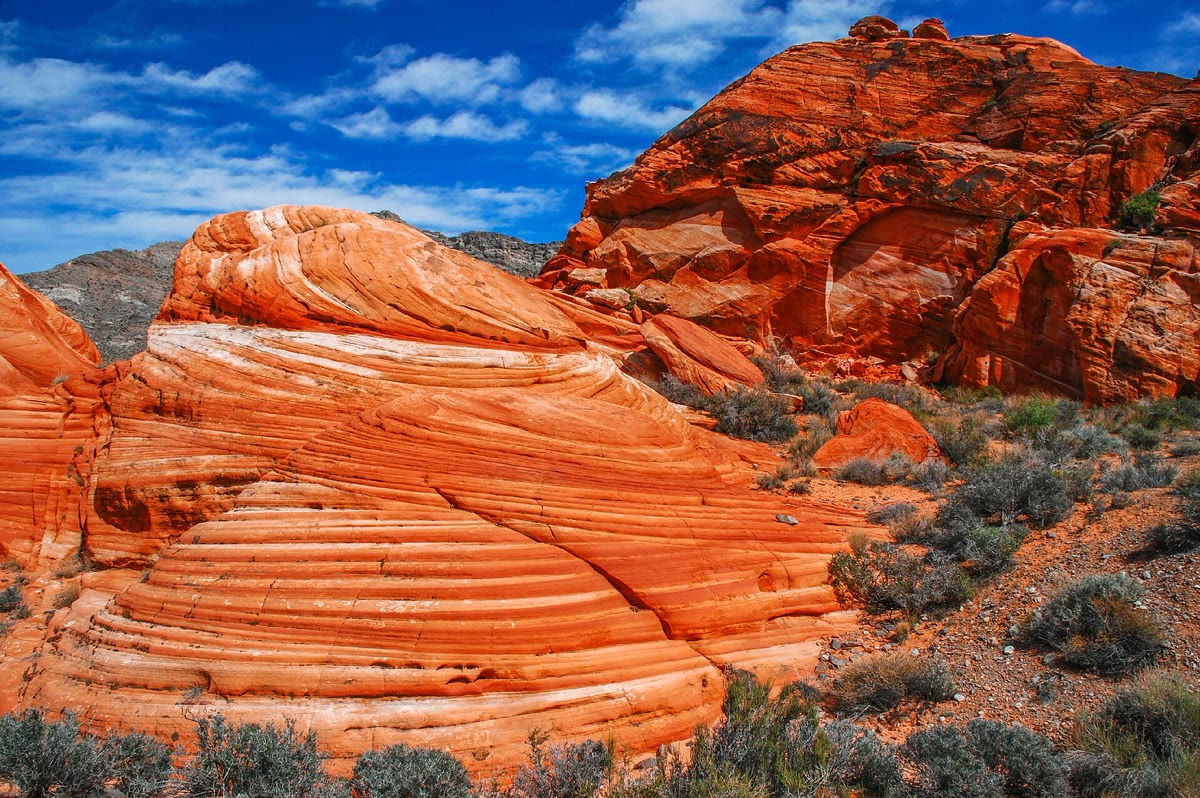
\includegraphics[height=3.6cm]{images/book3/b1-cross-bedding-aztec.jpg}};
\end{tikzpicture}

{\small يسارًا: هندسة أشكال القاع المتسلّقة (تخطيطي، والزوايا مبالغ فيها). تسير الأخاديد على مسارات مستقيمة مائلة بزاوية التسلّق $\theta$ (الخطوط السميكة)؛ وبين اثنين منها تُحفظ الأجزاء الدنيا من الواجهات الأمامية، في مجموعات سمكها $T = L\sin\theta$. ويمينًا: تطبّق متقاطع في حجر الرمل الأزتيكي، جبال موديّ، نيفادا: مجموعات مائلة من الصفائح، تقطع كلًّا منها من الأعلى سطحُ التآكل عند قاعدة التي تليها. صورة Chip Carroon, Bureau of Land Management, CC~BY-SA~2.0, عبر Wikimedia Commons.}
\label{fig:b1:clastic-sediments:climb}
\end{omfigure}
% ledger: southard:climb, commons:aztec-crossbed

\emph{التيارات القديمة.} تتشتّت اتجاهات \omterm{def:b1:geological-maps:attitude}{الانحدار} للتطبّقات المتقاطعة المقاسة على ظهور صخري حول الاتجاه المتوسط للتيار، لأن الوجوه المنحدرة للكثبان والتموّجات منحنية، وتتقلّب التيارات نفسها. ويُؤخذ متوسطها كمتوسط متجهي لا حسابي، للسبب المبيّن في \cref{prop:b1:field-lab-methods-1:vector-mean}: فالسموت زوايا على دائرة، والمتوسط بين 350 و\num{010} هو 000، لا 180.

\begin{proposition}[متوسط السموت]\label{prop:b1:clastic-sediments:azimuths}
لتكن $\alpha_1, \ldots, \alpha_N$ أسماتًا مقيسة في اتجاه عقارب الساعة من الشمال. فمتوسطها المتجهي $\bar\alpha$ ومتوسط طول محصّلتها $\bar R$ معطيان ب
\[
  S = \sum_{i=1}^N \sin\alpha_i, \quad C = \sum_{i=1}^N \cos\alpha_i, \quad
  \bar\alpha = \operatorname{atan2}(S, C), \quad \bar R = \frac{\sqrt{S^2 + C^2}}{N},
\]
حيث $\operatorname{atan2}(S, C)$ هي الزاوية التي يتناسب جيبها وجيب تمامها مع $S$ و$C$، وتُؤخذ بين \ang{0} و\ang{360}. و$\bar R$ يقع بين 0 و\num{1}، ولا يساوي 1 إلا إذا كانت كل الأسمات متساوية.
\end{proposition}

\begin{proof}
متجه الوحدة للسمت $\alpha$، مع الشرق إحداثيًّا أولًا والشمال إحداثيًّا ثانيًا، هو $(\sin\alpha, \cos\alpha)$. ومجموع المتجهات الوحدوية ال$N$ هو $(S, C)$، واتجاهه، أي المتوسط المتجهي (\cref{def:b1:field-lab-methods-1:mean-orientation})، له سمت جيبه وجيب تمامه $S/\sqrt{S^2+C^2}$ و$C/\sqrt{S^2+C^2}$. وبمتباينة المثلث يكون طول مجموع $N$ من المتجهات الوحدوية أقل من $N$ أو مساويًا له، ولا يساويه إلا حين تشير كلها إلى الاتجاه نفسه.
\end{proof}

\begin{method}[التيار القديم من التطبّق المتقاطع]\label{met:b1:clastic-sediments:palaeocurrent}
\begin{enumerate}
  \item على كل مجموعة، قِس \omterm{def:b1:geological-maps:attitude}{اتجاه الانحدار} للواجهات الأمامية، مختارًا أسطحًا تُظهر انحدارها الحقيقي (أو قِس \omterm{def:b1:geological-maps:attitude}{الامتداد} \omterm{def:b1:geological-maps:attitude}{والانحدار}).
  \item قِس \omterm{def:b1:geological-maps:attitude}{وضعية} التطبّق الرئيسي؛ فإن كان مائلًا بأكثر من بضع درجات، أعِد كل واجهة أمامية إلى الأفقي بالدوران حول امتداد التطبّق (دوران يُنجَز بالإسقاط الاستريوغرافي الوارد في مجلد السنة الثالثة).
  \item احسب المتوسط المتجهي $\bar\alpha$ و$\bar R$ لاتجاهات \omterm{def:b1:geological-maps:attitude}{الانحدار} المصحّحة (\cref{prop:b1:clastic-sediments:azimuths}).
  \item ارسم القراءات كمخطط الوردة، أي مدرّج تكراري دائري للسموت، لتعرف إن كانت تكوّن مجموعة واحدة أو مجموعتين: فالتيارات المدّية التي تنعكس تبني مجموعات تنحدر في اتجاهات متعاكسة، في تطبّق متقاطع على شكل عظمة السمكة، ويصير متوسط واحد عديم المعنى.
\end{enumerate}
\end{method}
% ledger: og:sorting-environments

\emph{بنى أخرى.} تسجّل بنى عدّة أخرى ظروف الترسيب واتجاه قمّة الطبقات. \omterm{def:b1:clastic-sediments:turbidite}{فالطبقة المتدرّجة} تنقص حبيباتها نحو الأعلى، من خشنة عند قاعدتها إلى ناعمة عند قمّتها، إذ تستقرّ الحبيبات من تيار يتراجع، والأخشن أولًا (\cref{def:b1:clastic-sediments:turbidite}). وتتكوّن تشقّقات الطين، أي شبكات مضلّعة من الشقوق الانكماشية تملؤها الطبقة التالية، حيث يجفّ الطين في الهواء، كما في الأراضي المدّية والسهول الفيضية. والحُفر التآكلية التي يحفرها التيار في الطين أسفله، ثم يملؤها الرمل فوقها، تُحفظ كقوالب على قاعدة طبقة الحجر الرملي، وأشكالها تشير إلى الاتجاه الذي سار فيه التيار.
% ledger: og:sorting-environments

\section{السحنات والأنهار والدلتاوات}\label{sec:b1:clastic-sediments:rivers-deltas}

يشكّل حجم الحبيبة \omterm{def:b1:clastic-sediments:sorting}{والفرز} والبنى والأحافير والتركيب معًا طابع الصخر الرسوبي، ويستعمل الجيولوجيون كلمة واحدة لذلك الطابع.

\begin{definition}[السحنة الرسوبية، والبيئة الترسيبية]\label{def:b1:clastic-sediments:facies}
\emph{السحنة الرسوبية}\index{السحنة الرسوبية} جسم من صخر رسوبي يتميّز عن غيره بصخريّته وحجم حبيباته وبنيته الرسوبية وأحافيره، وكلها تعكس الظروف التي تكوّن فيها. و\emph{البيئة الترسيبية}\index{البيئة الترسيبية} هي المكان، بظروفه الفيزيائية والكيميائية والحيوية، الذي يُرسَّب فيه الرسوب: مجرى نهر، أو سهل فيضي، أو شاطئ، أو منحدر دلتا، أو قاع البحر العميق.
\end{definition}
% ledger: og:sorting-environments

فالسحنة وصف، والبيئة تفسير، وقد تصنع عدّة بيئات السحنة نفسها: فالرمل المتموّج يترسّب في الأنهار وعلى الأوحال المدّية وعلى قاع البحر العميق. لذلك يرتكز التفسير على تجمّعات السحنات وعلى الترتيب الذي تتراكم به، وهذا الترتيب يتبع حركة البيئات في المكان: والقوانين العامة لهذا التراكب، والنماذج المعيارية لكل بيئة، موضوع مجلد السنة الثالثة. ويصف هذا الفصل البيئات الفتاتية الرئيسية والتعاقبات الرأسية التي تميّزها.

\emph{الأنهار المجدولة والمتعرّجة.} تأتي الأنهار في نمطين رئيسيين. النهر المجدول يجري في قنوات عديدة تنقسم وتلتقي من جديد حول حواجز من الحصى والرمل؛ والأنهار المجدولة تحمل حمولات خشنة قرب منابعها، تحت الجبال أو أمام الأنهار الجليدية، وترسباتها صفائح من الحصى ورمل خشن متطبّق متقاطع، بقليل من الطين. أما النهر المتعرّج فيجري في قناة واحدة ملتوية. وأسرع الماء يجري على خارج كل انعطاف، حيث يقضم الضفة المقطوعة؛ وعلى داخله، حيث الماء أبطأ، يترسّب الرمل على الحاجز الانعطافي. فينتقل الانعطاف جانبيًّا، يحفر من جهة ويبني على الأخرى؛ أما السهل الفيضي وراء الضفاف فلا يتلقّى سوى طين الفيضانات.
% ledger: og:rivers

ينتج تعاقب الحاجز الانعطافي عن أشكال القاع. فعند قاعدة الحاجز، في أعمق الماء وأسرعه، يترك التيار أخشن الحبيبات ويبني كثبانًا؛ وعلى الحاجز المنحدر برفق نحو الأعلى يصير الماء أضحل وأبطأ، والرمل أدقّ، وتُفسح الكثبان المجال للتموّجات (\cref{sec:b1:clastic-sediments:bedforms})؛ وفي القمّة يتحوّل الحاجز إلى السهل الفيضي. ومع هجرة الانعطاف تتحرّك كل من هذه المناطق فوق التي تحتها، فيلاقيها ثقب حفر يخترق الرسوب مكدّسة: تعاقب متناقص الحجم نحو الأعلى، من سطح تآكل إلى طين، لكل مرور لقناة، وسمكه نحو عمق القناة التي كوّنته.

\emph{الدلتاوات.} حيث يدخل النهر مسطّحًا مائيًّا راكدًا، يتفرّق تيارُه ويتباطأ، فتُسقط حمولته: الحمولة الخشنة قرب المصبّ، والناعمة أبعد. وينمو الدلتا إلى الأمام، أو يتقدّم، ما دام النهر يزوّده برسوب أكثر مما تستطيع الأمواج والمدّ حمله بعيدًا. وما تفعله الأمواج والمدّ بهذا الإمداد هو ما يحدّد شكله.

\begin{definition}[الدلتاوات التي تهيمن عليها الأنهار والأمواج والمدّ]\label{def:b1:clastic-sediments:delta}
تكون الدلتا \emph{نهرية الهيمنة}\index{دلتا نهرية الهيمنة} حين يطغى إمداد النهر على الأمواج والمدّ، وتبني قنواته المتفرّعة، المحصورة بأعرافها الطبيعية، أصابعَ طويلة من الرمل تمتدّ في البحر؛ وتكون \emph{أمواجية الهيمنة}\index{دلتا أمواجية الهيمنة} حين تعيد الأمواج تشكيل الرمل الواصل إلى المصبّات، فتبني شواطئ وحواجز شاطئية على ساحل أملس مقوّس؛ وتكون \emph{مدّية الهيمنة}\index{دلتا مدّية الهيمنة} حين تحمل تيارات المدّ الداخلة إلى المصبّات والخارجة منها الرمل إلى قضبان وحواجز موازية للجريان، مفصولة بقنوات على شكل قُمع.
\end{definition}
% ledger: og:deltas

\begin{omfigure}
\begin{tikzpicture}[font=\footnotesize, >={Stealth[length=4pt]}]
% meander in plan view (schematic) and the fining-upward log of a point bar
\begin{scope}[yscale=0.8]
  \fill[green!8] (-0.2,-0.4) rectangle (7.2,4.4);
  \draw[omSea!80!black, line width=9pt] plot[smooth, tension=0.7] coordinates {(0,3.6) (1.4,3.7) (2.6,2.8) (2.3,1.4) (3.2,0.5) (4.6,0.8) (5.0,2.2) (5.6,3.4) (7.0,3.5)};
  \draw[omSea!45, line width=7pt] plot[smooth, tension=0.7] coordinates {(0,3.6) (1.4,3.7) (2.6,2.8) (2.3,1.4) (3.2,0.5) (4.6,0.8) (5.0,2.2) (5.6,3.4) (7.0,3.5)};
  % point bars (inside of bends) with scroll lines
  \foreach \r in {0.25,0.45,0.65} {\draw[brown!60!black, densely dotted] (3.45,1.15) ++(200:\r) arc[start angle=200, end angle=340, radius=\r];}
  \fill[brown!25, opacity=0.8] (3.45,1.25) ellipse[x radius=0.55, y radius=0.35];
  \node[align=center] at (3.45,1.95) {الحاجز الانعطافي\\ (ترسيب)};
  \fill[brown!25, opacity=0.8] (1.75,2.75) ellipse[x radius=0.4, y radius=0.45];
  \node[align=center] at (1.3,1.95) {الحاجز الانعطافي};
  \draw[red!60!black, thick] (2.9,0.2) .. controls (3.3,0.0) and (4.3,0.15) .. (4.85,0.6);
  \node[red!60!black, anchor=north] at (4.0,0.0) {الضفة المقطوعة (تآكل)};
  \draw[->, black!70] (5.9,3.0) -- (6.7,3.15) node[right] {جريان};
  \node[anchor=north west, black!60] at (5.2,1.3) {السهل الفيضي};
  \node[font=\footnotesize] at (3.5,-0.85) {(أ) انعطاف، من الأعلى};
\end{scope}
\begin{scope}[xshift=9.2cm, yshift=-0.3cm, yscale=0.8]
  % log: x width = grain size; y = height
  \draw[lith shale] (0,3.6) rectangle (0.8,4.6);
  \draw[lith sandstone] (0,2.6) rectangle (1.2,3.6);
  \draw[lith sandstone] (0,0.6) rectangle (1.7,2.6);
  \draw[lith conglomerate] (0,0) rectangle (2.2,0.6);
  \draw[very thick, red!60!black] (0,0) -- (2.2,0);
  % cross-bed symbols
  \foreach \y in {0.9,1.5,2.1} {\draw[black!70] (0.3,\y) .. controls (0.6,\y+0.05) and (0.9,\y+0.25) .. (1.2,\y+0.4);}
  \foreach \x in {0.2,0.5,0.8} {\draw[black!70] (\x,3.0) -- ++(0.12,0.1) -- ++(0.12,-0.1);}
  \node[anchor=west, align=left] at (2.4,4.1) {طين السهل الفيضي،\\ جذور، تشقّقات طينية};
  \node[anchor=west, align=left] at (2.4,3.1) {رمل ناعم، تطبّق\\ متقاطع رقيق};
  \node[anchor=west, align=left] at (2.4,1.6) {رمل متوسط إلى خشن،\\ تطبّق متقاطع للكثبان};
  \node[anchor=west, align=left] at (2.4,0.3) {بقايا حصوية على\\ سطح تآكل};
  \draw[->] (-0.35,0) -- (-0.35,4.6) node[above] {أعلى};
  \draw[<->, black!60] (-0.7,0) -- node[above, rotate=90, font=\scriptsize] {عمق القناة} (-0.7,3.6);
  \node[font=\footnotesize] at (1.8,-0.5) {(ب) تعاقب الحاجز الانعطافي};
\end{scope}
\end{tikzpicture}

{\small (أ)~نهر متعرّج (تخطيطي): يحفر التيار الضفة الخارجية لكل انعطاف، ويترك الرمل على الحاجز الانعطافي في داخله؛ والخطوط المنحنية المتتابعة تمثّل المواقع المتعاقبة للحاجز. (ب)~التعاقب الذي يتركه حاجز انعطافي مهاجر، وعرض كل طبقة متناسب مع حجم حبيباتها (تخطيطي). وهو متناقص الحجم نحو الأعلى، وسمكه يسجّل عمق القناة.}
\label{fig:b1:clastic-sediments:point-bar}
\end{omfigure}
% ledger: og:rivers, southard:phase-diagram

تُوضع \omterm{def:b1:rock-forming-minerals:solid-solution}{الأطراف} الثلاثة عند رؤوس مثلث، يُوضع فيه أي دلتا بحسب القوّة النسبية للعمليات الثلاث. ودلتا المسيسيبي، ذو الأصابع الطويلة الممتدّة إلى خليج المكسيك على شكل قدم الطائر (\cref{ch:b1:erosion-transport})، هو النموذج الكلاسيكي \omterm{def:b1:clastic-sediments:delta}{لدلتا نهرية الهيمنة}؛ ودلتا النيل، بقوسه الملساء من الشواطئ، \omterm{def:b1:clastic-sediments:delta}{دلتا أمواجية الهيمنة}؛ ودلتا الغانج وبراهمابوترا، وهو الأكبر في العالم، \omterm{def:b1:clastic-sediments:delta}{دلتا مدّية الهيمنة}.
% ledger: og:deltas

\begin{omfigure}
\begin{tikzpicture}[font=\footnotesize]
% delta classification triangle (schematic) and the Lena delta from Landsat
\begin{scope}[yscale=0.82]
  \coordinate (R) at (2.6,4.5); \coordinate (W) at (0,0); \coordinate (T) at (5.2,0);
  \fill[omDef!8] (R) -- (W) -- (T) -- cycle;
  \draw[thick] (R) -- (W) -- (T) -- cycle;
  \node[above, align=center] at (R) {\textbf{نهرية الهيمنة}\\ أصابع مستطيلة، أعراف طبيعية};
  \node[below, align=center] at (W) {\textbf{أمواجية الهيمنة}\\ حواجز شاطئية ملساء};
  \node[below, align=center] at (T) {\textbf{مدّية الهيمنة}\\ قضبان موازية للجريان};
  \fill[omThm] (2.6,2.9) circle[radius=2pt] node[below=1pt] {مسيسيبي};
  \fill[omThm] (0.75,0.4) circle[radius=2pt] node[above right=0pt] {النيل};
  \fill[omThm] (4.4,0.4) circle[radius=2pt] node[above left=0pt, align=right] {الغانج--\\ براهمابوترا};
\end{scope}
\node[anchor=south west, inner sep=0] at (7.2,-0.9) {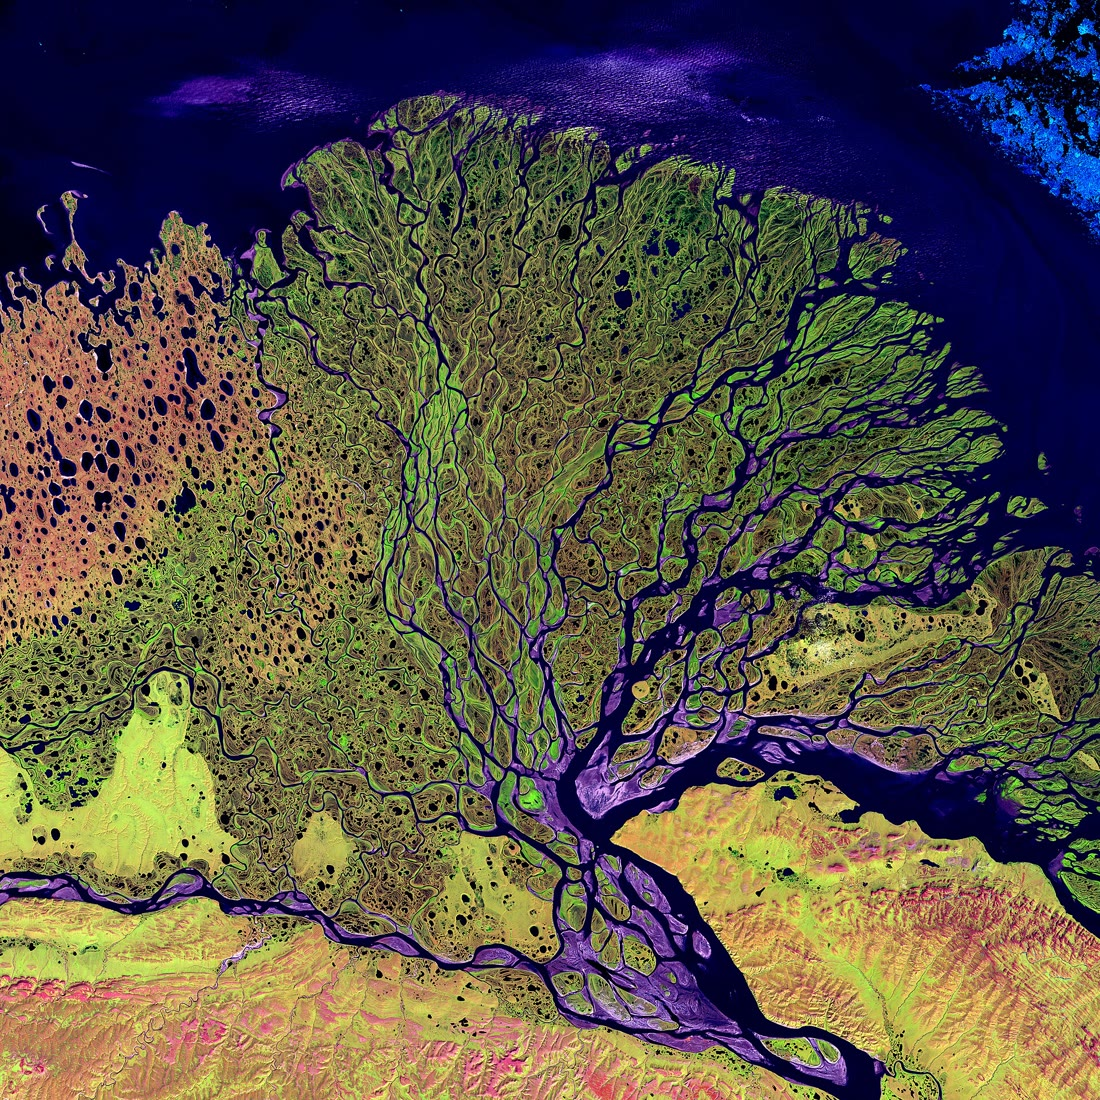
\includegraphics[height=5.2cm]{images/book3/b1-lena-delta.jpg}};
\end{tikzpicture}

{\small يسارًا: \omterm{def:b1:rock-forming-minerals:solid-solution}{الأطراف} الثلاثة للدلتاوات، بحسب العملية التي تشكّلها (تخطيطي؛ مواضع الأمثلة الثلاثة إرشادية). ويمينًا: دلتا لينا، في سيبيريا، المبنية في بحر لابتيف (أعلى)؛ يدخل النهر من الركن الأيمن السفلي ويتفرّع إلى مئات الفروع. صورة كاذبة الألوان من Landsat~7 بتاريخ 27 فبراير 2000، U.S. Geological Survey, ملك عام، عبر Wikimedia Commons.}
\label{fig:b1:clastic-sediments:deltas}
\end{omfigure}
% ledger: og:deltas, commons:lena-delta

\emph{التعاقب المتزايد الخشونة نحو الأعلى.} أمام مصبّ النهر تملك الدلتا واجهةً منحدرة برفق، هي واجهة الدلتا، تتّصل نحو البحر بما قبل الدلتا، حيث يستقرّ الطين وحده من التعليق. ومع تقدّم الدلتا يتقدّم كل من هذه المناطق فوق التي أمامه: فثقب حفر على سهل الدلتا يلاقي، من الأسفل إلى الأعلى، طين ما قبل الدلتا الصفائحي، ثم طميًا ورملًا متناوبين من الواجهة السفلى للدلتا، ثم رملًا متطبّقًا متقاطعًا من حواجز المصبّ، تقطعه في الأعلى قنوات سهل الدلتا. ويتزايد التعاقب خشونةً نحو الأعلى، عكس الحاجز الانعطافي، وسمكه يقارب عمق الماء الذي بنى فيه الدلتا. ومعدّل بنائه مرتبط بهندسة واجهة الدلتا.

\begin{proposition}[التقدّم والتراكم]\label{prop:b1:clastic-sediments:progradation}
لتكن واجهة دلتا ذات ميل ثابت $\alpha$ تتقدّم أفقيًّا بالسرعة $v$ دون أن تتغيّر هيئتها، عند مستوى بحر ثابت. فنقطة ثابتة تحت الواجهة تتلقّى عندئذٍ رسوبًا بالمعدّل الرأسي
\[
  a = v\,\tan\alpha,
\]
ويتراكم هناك تعاقب واجهة الدلتا، سمكه $h$، في الزمن $h/(v\tan\alpha)$.
\end{proposition}

\begin{proof}
في الزمن $\mathrm dt$ تتقدّم الواجهة إلى الأمام بمقدار $v\,\mathrm dt$. وعند نقطة ثابتة تحت السطح المنحدر يرتفع السطح بفرق الارتفاع بين نقطتين من الواجهة تبعدان أفقيًّا $v\,\mathrm dt$، أي $v\,\mathrm dt\,\tan\alpha$، ومن ثمّ المعدّل. وتمرّ الواجهة بالنقطة بينما يرتفع السطح بمقدار $h$، وذلك يستغرق الزمن $h/a$.
\end{proof}

تنحدر واجهات الدلتا برفق، ف$\tan\alpha$ صغيرة: تتقدّم واجهة الدلتا أسرع بكثير من تراكم الرسوب عند أيّ نقطة تحتها (\cref{exo:b1:clastic-sediments:12}).

\begin{inthelab}[وصف لبّ الحفر]
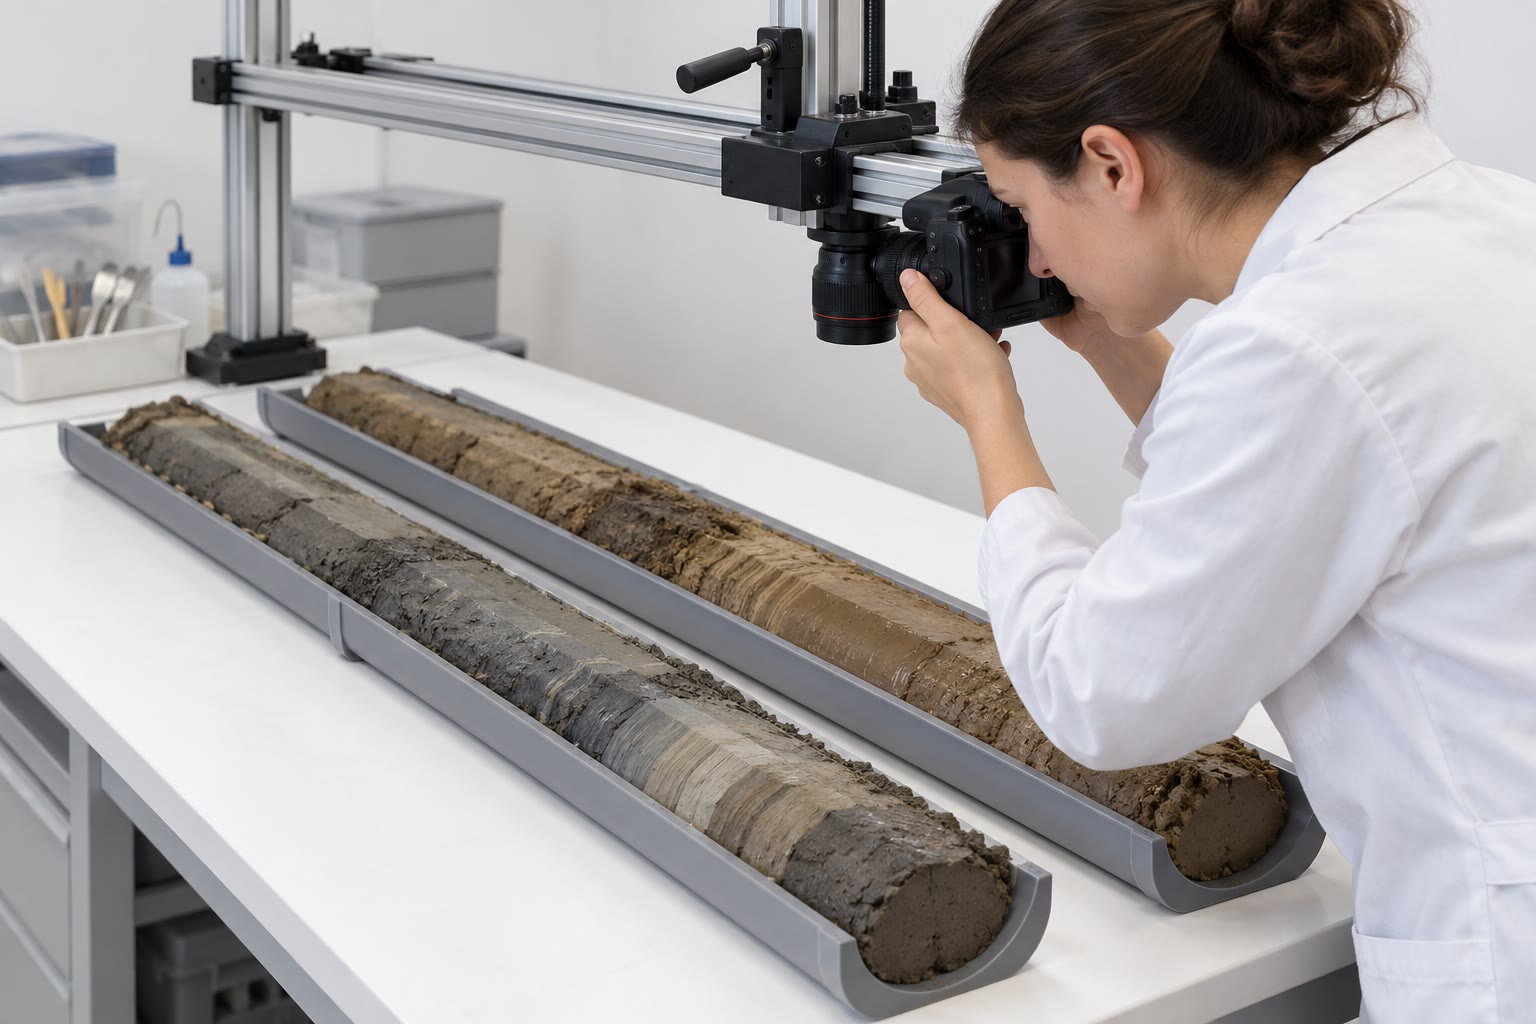
\includegraphics[width=0.3\linewidth]{images/book3/ai/b1-core-lab.jpg}\hfill
\begin{minipage}[b]{0.67\linewidth}
تُوضع الأسطوانات من الرسوب أو الصخر التي يُخرجها المثقاب في صوانٍ بحسب العمق، وتُشقّ طوليًّا، وتُصوَّر تحت إضاءة متساوية قبل أن تجفّ وتتغيّر ألوانها. ثم يرسم عالم الرسوبيات سجلًّا للبّ، متًرًا بمتر: الصخريّة، وحجم حبيبات كل طبقة (عرض العمود)، والبنى (تطبّق متقاطع، والتصفيح، والتدرّج، والثقوب الحيوانية)، وحدود \omterm{def:b1:geological-maps:geological-map}{التماس}، حادّة كانت أو تدريجية، واللون، والأحافير. وتُؤخذ عينات لتحليل حجم الحبيبات والشرائح الرقيقة. فاللبّ نافذة ضيّقة واحدة: اتجاه التطبّقات المتقاطعة يضيع إن لم يكن اللبّ موجَّهًا، ويجب أن يأتي \omterm{def:b1:geological-maps:attitude}{الامتداد} الجانبي للطبقات من حفرات أخرى.
\end{minipage}

\smallskip
{\small لبّ موضوع لتصويره في مختبر رسوبيات (توضيحي بالذكاء الاصطناعي).}
\end{inthelab}

\section{الشاطئ والرفّ القاري}\label{sec:b1:clastic-sediments:shoreline}

على طول الساحل بين الدلتاوات، يُعاد تشكيل الرمل الذي تجلبه الأنهار بفعل الأمواج والمدّ. والشاطئ رمل أعادت تشكيله الغسلة، أي الصفيحة الرقيقة من الماء التي تندفع صعودًا وهبوطًا عليه بعد كسر كل موجة: فتُنقل الحبيبات مرارًا وتكرارًا، وتُحمل الناعمة منها إلى البحر، وتكون رمال الشواطئ من أفضل الرسوبيات فرزًا وأكثرها استدارة. وصفائحها التي ترسبها الغسلة تنحدر نحو البحر برفق. وعلى كثير من السواحل المنخفضة يكوّن الرمل جُزرًا حاجزية، وهي حواجز طويلة من شاطئ وكثبان ريحية، تفصلها عن البرّ بحيرات هادئة دقيقة الحبيبات، تتّصل بالبحر عبر مداخل مدّية.

وحيث تكون المدّ قوية والأمواج ضعيفة، يحيط بالساحل أوحال مدّية، تغمرها المياه وتكشفها مرتين في اليوم. وتتدرّج من الرمل قرب خطّ الجزر، حيث التيارات أقوى، إلى الطين قرب خطّ المدّ، حيث يسمح الماء الراكد للطين بالاستقرار؛ وتُظهر رسوباتها الجريان المتعاكس في تطبّق متقاطع على شكل عظمة السمكة، وجفاف الطين في تشقّقات طينية، وتناوب التيار والماء الراكد في طبقات طينية رقيقة مُسدَلة على رمل متموّج.

وفي البحر، يُكتسح الرفّ القاري بالأمواج حتى عمق يزيد مع حجم الأمواج. فوقه يُنقل الرمل ويُغربَل؛ وتحته يترسّب الطين، إلا أثناء العواصف، حين تصل الأمواج الأكبر إلى أعماق أكبر فتترك صفائح من الرمل ذات تصفيح حَدَبي لطيف يُسمّى \omterm{def:b1:clastic-sediments:cross-bedding}{التطبّق المتقاطع} الحَدَبي. وهكذا يتناوب تعاقب الرفّ كثيرًا الطينَ في الطقس الهادئ مع رمال العواصف، وتكون الطبقات أسمك وأخشن نحو الشاطئ.
% ledger: og:sorting-environments, folk:maturity

\section{الرسوبيات الفتاتية في أعماق البحر}\label{sec:b1:clastic-sediments:deep-sea}

ويصل الرمل والحصى أيضًا إلى قيعان المحيطات العميقة، على آلاف الأمتار من العمق ومئات الكيلومترات بعيدًا عن اليابسة، وتنقلهما إلى هناك تيارات لم يرها أحد بتمامها: تيارات كثيفة محمّلة بالرسوبيات تهبط على المنحدر القاري تحت المياه الصافية للمحيط.

\begin{history}[كابلات قاع البحر، 1929]
في 18 نوفمبر 1929 ضرب زلزال بمقدار العزم 7.2 منحدرَ القارة جنوب نيوفاوندلاند، على الحافة الجنوبية لبنك غراند. انزلقت على المنحدر كتلة تقارب \qty{200}{km^3} من الرسوبيات، وقتل تسونامي 28 شخصًا على ساحل نيوفاوندلاند. وانقطعت اثنتا عشرة كابلًا تلغرافيًّا مُدّت عبر قاع البحر، بعضها في عدّة مواضع. أما القريبة من المركز فانقطعت في الحال؛ والبقية، أبعد جنوبًا وأعمق، انقطعت الواحدة بعد الأخرى في الساعات التالية، بترتيب بُعدها على طول المنحدر. وفي 1952 فسّرها بروس هيزن وموريس إيوينغ، وهما يدرسان أوقات الانقطاع: فقد تحوّل الانزلاق إلى \omterm{def:b1:clastic-sediments:turbidite}{تيار العكارة} جرى على المنحدر ثم عبر السهل القاعي العميق مسافةً تزيد على 480 ميلًا، قاطعًا كل كابل يمرّ به. ومن الأوقات والمسافات قدّرا سرعته بنحو 50 عقدة على الجزء الأعلى من منحدر القارة، حيث الميل نحو \qty{0.5}{\percent}، ولا تزال 12 عقدة عند آخر كابل، على نحو 400 ميل من منشئه. ومع تباطئه، زعما، كان لا بدّ أن يُرسّب على السهل طبقة متدرّجة تزداد نعومتها كلما صعدت.
\end{history}
% ledger: nrcan:grand-banks, he52:grand-banks

50 عقدة تساوي \qty{25.7}{m.s^{-1}}، أي أكثر من \qty{90}{km.h^{-1}}، سرعة سيارة على طريق رئيسي؛ و\num{12} عقدة تساوي \qty{6.2}{m.s^{-1}}؛ و\num{480} ميلًا تساوي نحو \qty{770}{km}. وأعطت الانقطاعات كذلك أولى السرعات المقاسة لتيار لم يُستنتج إلا من رسوباته ومن تجارب الأحواض.
% ledger: he52:grand-banks

\begin{definition}[تيار العكارة، والعكرة، والطبقة المتدرّجة]\label{def:b1:clastic-sediments:turbidite}
\emph{تيار العكارة}\index{تيار العكارة} تيار من ماء صار أثقل من الماء المحيط به بسبب الرسوب الذي يحمله معلّقًا، يجري نزولًا على منحدر تحت ذلك الماء، وحبيباته معلّقة بفعل الاضطراب الذي تولّده حركته. و\emph{العكرة}\index{العكرة} هي الرسوب الذي يتركه تيار العكارة. و\emph{الطبقة المتدرّجة}\index{الطبقة المتدرّجة} طبقة يتناقص حجم حبيباتها من قاعدتها إلى قمّتها.
\end{definition}
% ledger: og:sorting-environments, he52:grand-banks

يدفع \omterm{def:b1:clastic-sediments:turbidite}{تيار العكارة} نفسه بنفسه: فهو يجري لأن تعليقه ثقيل، ويحافظ على تعليقه لأنه يجري. فعلى منحدر شديد يلتقط مزيدًا من الرسوب من القاع، فيزداد كثافةً ويتسارع؛ وعلى المنحدر الرفيق للسهل القاعي يتباطأ، فيُسقط حمولته ويتلاشى.

\begin{proposition}[سرعة تيار العكارة]\label{prop:b1:clastic-sediments:turbidity}
تيار عكارة سماكته $h$ وكثافته $\rho + \Delta\rho$ يجري بانتظام نزولًا على منحدر ميله $S$ تحت ماء كثافته $\rho$. فإذا كانت مقاومة القاع والماء الذي فوقه $\tau = \rho\,C_f\,U^2$ لكل وحدة مساحة، وكان $C_f$ معامل احتكاك بلا بعد، فإن سرعته المتوسطة هي
\[
  U = \sqrt{\frac{\Delta\rho}{\rho}\,\frac{g\,h\,S}{C_f}} .
\]
\end{proposition}

\begin{proof}
يقوم البرهان على حاصل العمق والميل (\cref{prop:b1:erosion-transport:depth-slope})، مع استبدال الوزن بالوزن الزائد. وعمود من التيار مساحته الوحدة يزن $(\rho +
\Delta\rho) g h$، والماء الذي يزيحه $\rho g h$: فلا يجذبه نحو أسفل المنحدر في الماء المحيط سوى الزيادة $\Delta\rho\,g\,h$، بمركّبة $\Delta\rho\,g\,h\,S$ على طوله. وفي الجريان المستقر توازن هذه المركّبة المقاومة $\rho C_f U^2$، ومن ثمّ $U^2 = (\Delta\rho/\rho)\,g\,h\,S/C_f$.
\end{proof}

قانون المقاومة $\tau = \rho C_f U^2$، التربيعي في السرعة، هو قانون الجريانات المضطربة في الهيدروليك (كتب الفيزياء)، و$C_f$ يُوجد بالتجربة. والصيغة تُهمل الماء الذي يمزجه التيار بنفسه عبر سطحه العلوي، فيخفّفه ويبطّئه. وهي تبيّن دور العوامل الثلاثة: تيار أسمك، أو أكثف، أو على منحدر أشدّ ميلًا بمرّتين، يجري أسرع ب$\sqrt 2$ مرة. ومعلّق يحمل كسر $c$ من حجمه حبيبات كوارتز له $\Delta\rho/\rho = 1.65\,c$ (\cref{sec:b1:erosion-transport:settling})، وهو صغير إلا إن كان الجريان مركّزًا جدًّا؛ وهنا يختلف \omterm{def:b1:clastic-sediments:turbidite}{تيار العكارة} عن النهر، الذي يدفعه الوزن الكامل للماء، لا فائض صغير منه. ولكي يجري بسرعة 50 عقدة كما في 1929 على منحدر ميله \qty{0.5}{\percent}، يحتاج \omterm{def:b1:clastic-sediments:turbidite}{تيار العكارة} إلى حاصل كبير من السمك وفائض الكثافة (\cref{exo:b1:clastic-sediments:11}).

\emph{تسلسل بوما.} في 1962 وصف أرنولد بوما الترتيب الداخلي لطبقات الحجر الرملي في تعاقبات أعماق البحار القديمة، في خمسة أقسام تُعنون من الأسفل إلى الأعلى. A: رمل كتلي أو متدرّج، غالبًا على قاعدة تآكلية؛ B: رمل ذو تصفيح متوازٍ؛ C: رمل ناعم بتصفيح متقاطع للتموّجات، غالبًا ملتوٍ؛ D: طمي مصفّح يتدرّج إلى طين؛ E: طين. ويُقرأ الترتيب كسجلّ لتيار واحد يتراجع يمرّ فوق نقطة: فحين يتباطأ يُسقط أولًا أخشن حبيباته دفعةً واحدة، ثم يبني قاعًا مستويًا علويًّا، ثم تموّجات، ثم يترك الطمي والطين يستقرّان. والتعاقبات الكاملة نادرة: فالأقسام العليا كثيرًا ما يحفرها التيار التالي، وبعيدًا عن المصدر، حيث التيار ضعيف، تغيب الأقسام السفلى.
% ledger: og:sorting-environments, shanmugam:bouma

\begin{omfigure}
\begin{tikzpicture}[font=\footnotesize]
% Bouma sequence: log (schematic) and a labelled photograph
\begin{scope}
  \draw[lith shale] (0,4.0) rectangle (0.7,4.8);
  \draw[lith shale] (0,3.3) rectangle (0.9,4.0);
  \draw[lith sandstone] (0,2.2) rectangle (1.3,3.3);
  \draw[lith sandstone] (0,1.2) rectangle (1.6,2.2);
  \draw[lith sandstone] (0,0) rectangle (2.0,1.2);
  \draw[very thick, red!60!black] (0,0) .. controls (0.6,-0.12) and (1.4,0.1) .. (2.0,0);
  \foreach \y in {1.4,1.6,1.8,2.0} {\draw[black!70] (0.1,\y) -- (1.5,\y);}
  \foreach \x in {0.15,0.5,0.85} {\draw[black!70] (\x,2.55) .. controls (\x+0.12,2.75) .. (\x+0.3,2.6);}
  \foreach \y in {3.45,3.6,3.75,3.9} {\draw[black!60] (0.1,\y) -- (0.8,\y);}
  \foreach \x/\y in {0.4/0.3, 0.9/0.5, 1.4/0.25, 0.6/0.8, 1.2/0.9} {\fill[black!60] (\x,\y) circle[radius=0.06];}
  \node[anchor=west] at (2.2,4.4) {E \quad طين};
  \node[anchor=west] at (2.2,3.65) {D \quad طمي مصفّح يتدرّج إلى طين};
  \node[anchor=west] at (2.2,2.75) {C \quad تصفيح متقاطع للتموّجات};
  \node[anchor=west] at (2.2,1.7) {B \quad تصفيح متوازٍ};
  \node[anchor=west] at (2.2,0.6) {A \quad رمل متدرّج};
  \node[anchor=west, red!60!black] at (2.2,-0.15) {قاعدة تآكلية، علامات قاع};
  \draw[->] (-0.3,0) -- (-0.3,4.8) node[above] {أعلى};
\end{scope}
\node[anchor=south west, inner sep=0] at (6.9,-0.3) {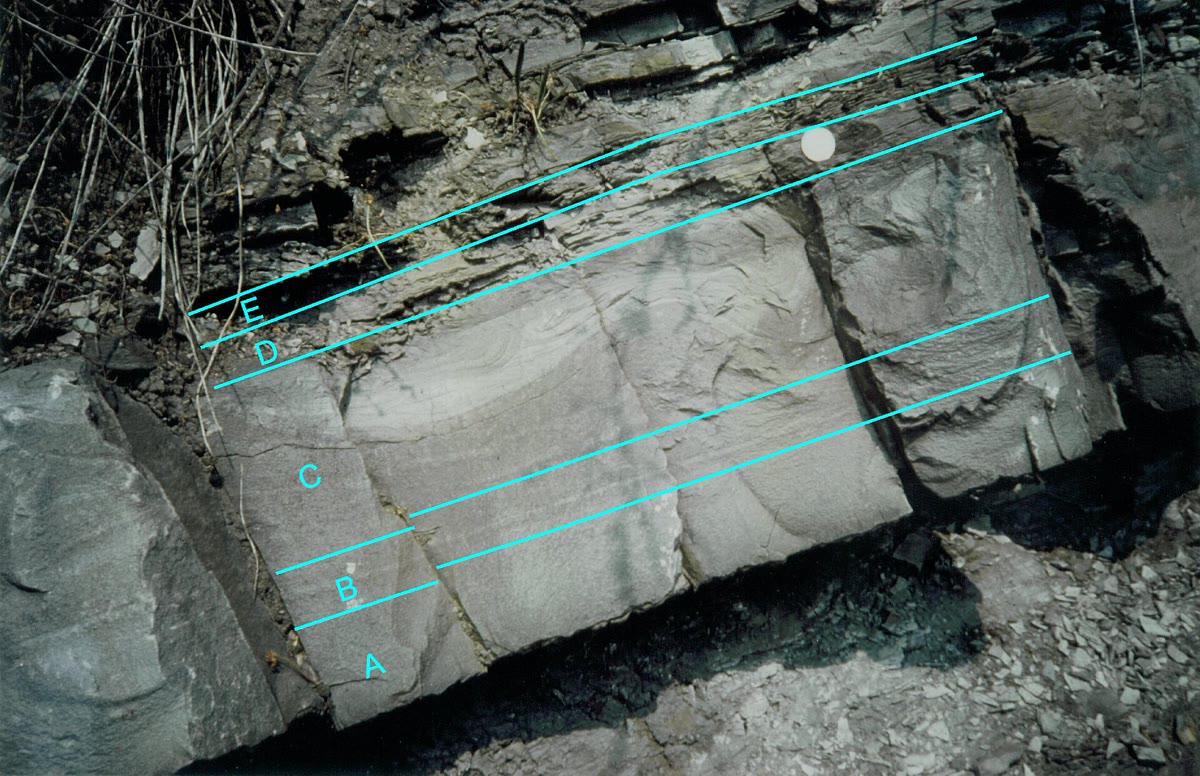
\includegraphics[height=5.2cm]{images/book3/b1-turbidite-bouma.jpg}};
\end{tikzpicture}

{\small يسارًا: أقسام تسلسل بوما الخمسة، وعرض كل منها متناسب مع حجم حبيباته (تخطيطي). ويمينًا: طبقة عكرة من الديفوني الأعلى في بيكه-أوزه، ألمانيا، وقد وسم المصوّر الأقسام من A إلى E؛ والقطعة النقدية تعطي المقياس. صورة Jo Weber, CC~BY-SA~3.0, عبر Wikimedia Commons.}
\label{fig:b1:clastic-sediments:bouma}
\end{omfigure}
% ledger: og:sorting-environments, shanmugam:bouma, commons:bouma-becke-oese

أصبح تسلسل بوما النموذج المعياري للعكَر، وفُسّرت به آلاف الحجارة الرملية العميقة القديمة. والتفسير محلّ جدل: فالتيارات الجارية على طول المنحدر، والتيارات المدّية العميقة، والأمواج الداخلية، تبني أيضًا رمالًا متموّجة ومصفّحة، ويرى بعض الرسوبيين أن كثيرًا من الطبقات المقروءة كعَكَر، بما فيها بعض طبقات المنطقة النموذجية، رسبتها تيارات أخرى. ونادرًا ما رُصدت تيارات العكارة في المحيط الحديث، بينما تُعدّ العكَر القديمة بالآلاف.
% ledger: shanmugam:bouma

ولا تُمثّل كل الرسوبيات الفتاتية في أعماق البحار عكَرًا. فتيارات الكنتور، وهي التيارات البطيئة العميقة التي تتبع خطوط الكنتور للمنحدر القاري، تعيد تشكيل رسوب المنحدر إلى ركامات مستطيلة ملساء تُسمّى الكونتوريتات. وبعيدًا عن القارات، حيث لا تصل لا تيارات العكارة ولا تيارات الكنتور، لا يتلقّى قاع البحر سوى ما يهبط من الماء الذي فوقه: أصداف العوالق والغبار الريحي الأدقّ، وهي الرسوبيات البيلاجية في الفصل التالي (\cref{ch:b1:chemical-biogenic-sediments}).
% ledger: og:sorting-environments

\section{التمارين}

\begin{exercise}[$\star$]\label{exo:b1:clastic-sediments:1}
حوّل إلى وحدات فاي الأقطار \qty{0.18}{mm}، و\qty{0.75}{mm}، و\qty{3}{mm}، و\qty{0.012}{mm}، و\qty{150}{mm}، إلى منزلتين عشريتين، وسمِّ صنف كل منها (\cref{tab:b1:clastic-sediments:classes}).
% ledger: folk:wentworth-classes
\end{exercise}

\begin{exercise}[$\star$]\label{exo:b1:clastic-sediments:2}
يعطي المنحنى التراكمي لرمل نهري $\varphi_5 = 0.62$، و$\varphi_{16} =
1.05$، و$\varphi_{50} = 1.71$، و$\varphi_{84} = 2.43$، و$\varphi_{95} = 2.98$. احسب متوسطه البياني، بوحدات فاي وبالمليمترات، وانحرافه المعياري البياني الشامل، وسمِّ حجمه وفرزه.
% ledger: folk:graphic-measures, folk:sorting-classes
\end{exercise}

\begin{exercise}[$\star$]\label{exo:b1:clastic-sediments:3}
تموّجات ارتفاعها \qty{2}{cm} تتحرّك بسرعة \qty{1}{cm} في الدقيقة فوق قاع من رمل كوارتزي مساميته \num{0.4}. باستعمال \cref{prop:b1:clastic-sediments:migration}، احسب حجم \omterm{def:b1:erosion-transport:load}{الحمولة القاعية} لكل وحدة عرض، بالوحدة \si{m^2.s^{-1}}، وكتلة الكوارتز ($\qty{2650}{kg.m^{-3}}$) المحمولة فوق متر من القمّة في يوم.
% ledger: hom:quartz
\end{exercise}

\begin{exercise}[$\star$]\label{exo:b1:clastic-sediments:4}
العقدة ميل بحري واحد، \qty{1852}{m}، في الساعة. (أ)~حوّل إلى أمتار في الثانية السرعتين 50 و\num{12} عقدة المقدّرتين \omterm{def:b1:clastic-sediments:turbidite}{لتيار العكارة} في 1929. (ب)~كم يستغرق تيار بسرعة 12 عقدة ليقطع \qty{100}{km}؟ (ج)~حوّل 480 و\num{400} ميل إلى كيلومترات (الميل الواحد \qty{1.609}{km}).
% ledger: he52:grand-banks
\end{exercise}

\begin{exercise}[$\star\star$]\label{exo:b1:clastic-sediments:5}
(أ)~باستعمال النسب المئوية لتوزيع طبيعي المعطاة في برهان \cref{prop:b1:clastic-sediments:normal}، احسب الانحراف المعياري البياني $(\varphi_{84} - \varphi_{16})/2$، والتقدير $(\varphi_{95} - \varphi_5)/3.3$ لتوزيع طبيعي انحرافه المعياري $\sigma$. (ب)~لماذا قد يختلف الاثنان في رسوب حقيقي؟ وأيّ نوع من الرسوبيات يجعلهما يختلفان أكثر؟
\end{exercise}

\begin{exercise}[$\star\star$]\label{exo:b1:clastic-sediments:6}
تُظهر طبقات من تموّجات متسلّقة مجموعات سمكها \qty{1.5}{cm}، مقيسًا عموديًّا على حدودها، تكوّنها تموّجات متباعدة ب\qty{15}{cm}. (أ)~احسب زاوية التسلّق. (ب)~إن تحرّكت التموّجات بسرعة \qty{0.5}{cm} في الدقيقة، فبأيّ معدّل رُفع القاع، بالسنتيمترات في الساعة؟ (ج)~ماذا يقول مثل هذا المعدّل عن الجريان؟
% ledger: southard:climb
\end{exercise}

\begin{exercise}[$\star\star$]\label{exo:b1:clastic-sediments:7}
ستّ اتجاهات انحدار للتطبّقات المتقاطعة، مصحّحة لميل الطبقات، قرأت 350 و\num{020} و\num{005} و\num{340} و\num{015} و\num{030}. (أ)~احسب متوسطها الحسابي. (ب)~احسب متوسطها المتجهي و$\bar R$. (ج)~فسّر الفرق.
\end{exercise}

\begin{exercise}[$\star\star$]\label{exo:b1:clastic-sediments:8}
فُحصت ثلاثة حجارة رملية في شريحة رقيقة. فالحجر A فيه \qty{12}{\percent} من أرضية طينية، وحبيبات كوارتز زاوية \omterm{def:b1:rock-forming-minerals:groups}{والفلسبار} وأجزاء صخرية. وفي B \qty{2}{\percent} من الطين، و$\sigma_I = 0.40\,\varphi$، وحبيبات كوارتز بدرجة استدارة \num{2.2} على مقياس فولك. وC لا طين فيه، و$\sigma_I =
0.30\,\varphi$، وحبيبات كوارتز بدرجة استدارة \num{3.6}، و\qty{98}{\percent} كوارتز. سمِّ \omterm{def:b1:clastic-sediments:maturity}{النضج النسيجي} لكل منها، واقترح بيئة ترسيب لكل منها.
% ledger: folk:maturity
\end{exercise}

\begin{exercise}[$\star\star$]\label{exo:b1:clastic-sediments:9}
(أ)~احسب عدد فرود لجريان عمقه \qty{0.3}{m} بسرعة \qty{1.5}{m.s^{-1}}، ولنهر عمقه \qty{2}{m} بسرعة \qty{1.0}{m.s^{-1}} ($g
= \qty{9.81}{m.s^{-2}}$). (ب)~عند أيّ عمق يبلغ جريان بسرعة \qty{1.5}{m.s^{-1}} عدد فرود 1، وأيّ سرعة يحتاجها نهر عمقه \qty{2}{m}؟ (ج)~لماذا تكثر المضادات للكثبان في صفائح الماء الجارية عن شاطئ، وتندر في الأنهار الكبيرة؟
% ledger: southard:ripples-dunes
\end{exercise}

\begin{exercise}[$\star\star\star$]\label{exo:b1:clastic-sediments:10}
أعطى تحليل غربالي لرمل، في فئات فاي كاملة من $-1$ إلى $5\,\varphi$: 2، و\num{8}، و\num{30}، و\num{40}، و\num{15}، و\num{5} بالوزن في المئة. (أ)~بطريقة العزوم، احسب المتوسط والانحراف المعياري بوحدات فاي، وسمِّ \omterm{def:b1:clastic-sediments:sorting}{الفرز}. (ب)~ارسم المنحنى التراكمي، واقرأ $\varphi_5$، و$\varphi_{16}$، و$\varphi_{50}$، و$\varphi_{84}$، و$\varphi_{95}$ بالاستيفاء الخطّي، واحسب $M_z$ و$\sigma_I$. (ج)~قارن.
% ledger: folk:graphic-measures, folk:sorting-classes
\end{exercise}

\begin{exercise}[$\star\star\star$]\label{exo:b1:clastic-sediments:11}
خذ $C_f = 0.003$ في \cref{prop:b1:clastic-sediments:turbidity}. (أ)~تيار عكارة سمكه \qty{50}{m}، وفائض كثافته \qty{2}{\percent}، يجري على منحدر ميله \num{0.005}: احسب سرعته بالأمتار في الثانية وبالعقد. (ب)~ما حاصل السمك وفائض الكثافة النسبي الذي يعطي 50 عقدة في 1929 على المنحدر نفسه؟ (ج)~يصل التيار نفسه في (أ) إلى منحدر ميله \num{0.001}: احسب سرعته الجديدة إن لم يتغيّر شيء آخر. ماذا يحدث لحمولته؟
% ledger: he52:grand-banks
\end{exercise}

\begin{exercise}[$\star\star\star$]\label{exo:b1:clastic-sediments:12}
يحمل نهر \qty{50}{Mt} من الرسوبيات في السنة إلى دلتاه، منها \qty{70}{\percent} تترسّب على واجهة دلتا عرضها \qty{100}{km} تبني في ماء عمقه \qty{30}{m}. وكثافة الرسوب الحجمية \qty{2000}{kg.m^{-3}}. (أ)~ما الحجم الذي تضيفه كل سنة؟ (ب)~إن ملأ هذا الحجم كامل عمق الماء على عرض الواجهة، فبأيّ سرعة تتقدّم الواجهة؟ (ج)~مع ميل واجهة الدلتا \ang{0.5}، بأيّ معدّل يتراكم الرسوب عند نقطة ثابتة تحت الواجهة، وفي كم سنة يتكوّن هناك التعاقب المتزايد الخشونة نحو الأعلى؟
\end{exercise}

\section{مسألة: قراءة لبّ من دلتا}

\begin{problem}[{مسألة نهاية الأسبوع --- ثقب حفر عبر دلتا قديمة، من أحجام الحبيبات إلى اتجاه أنهارها}]
\label{pb:b1:clastic-sediments:1}
% values: calc/ch21.py; the borehole, its beds, ages and readings are invented
يعبر ثقب حفر \qty{24}{m} من الحجارة الرملية والطينية التي رسّبتها دلتا قديمة. يصف الجيولوجي أربع وحدات، من القاعدة إلى الأعلى، ويحلّل عيّنة من كل منها.

\smallskip
\begin{center}\small
\begin{tabular}{@{}llccccc@{}}
\hline
الوحدة (العمق من القاعدة) & الوصف & $\varphi_5$ & $\varphi_{16}$ & $\varphi_{50}$ & $\varphi_{84}$ & $\varphi_{95}$ \\
\hline
1 (0--8 m) & حجر طيني رمادي مصفّح & 4.2 & 5.0 & 6.6 & 8.4 & 9.6 \\
2 (8--16 m) & حجر طمي وحجر رملي متناوبان & 1.9 & 2.4 & 3.4 & 4.6 & 5.5 \\
3 (16--21 m) & حجر رملي متطبّق متقاطع & 0.9 & 1.25 & 1.8 & 2.35 & 2.7 \\
4 (21--24 m) & حجر رملي حصوي، قاعدة تآكلية & $-1.8$ & $-0.8$ & 0.9 & 2.1 & 2.9 \\
\hline
\end{tabular}
\end{center}

\medskip
\noindent\textbf{الجزء الأول --- الحبيبات.}
\begin{enumerate}
  \item احسب المتوسط البياني $M_z$ لكل وحدة، بوحدات فاي وبالمليمترات.
  \item احسب الانحراف المعياري البياني الشامل $\sigma_I$ لكل وحدة.
  \item سمِّ صنف حجم المتوسط \omterm{def:b1:clastic-sediments:sorting}{والفرز} لكل وحدة.
  \item أيّ الوحدات أفضل فرزًا؟ ولماذا يكون حاجز المصبّ أفضل فرزًا من طين ما قبل الدلتا؟
  \item بالاستيفاء الخطّي بين $\varphi_{50}$ و$\varphi_{84}$، قدّر النسبة المئوية للجسيمات بحجم الطين (الأدقّ من $8\,\varphi$) في الوحدة~1. ماذا تقول عن التيارات التي رسّبتها؟
  \item لماذا يكون المنحنى التراكمي للوحدة~4 منتشرًا بهذا الشكل، مع أنها رمل قناة؟
\end{enumerate}

\medskip
\noindent\textbf{الجزء الثاني --- التعاقب.}
\begin{enumerate}[resume]
  \item صِف كيف يتغيّر الحجم المتوسط من الوحدة~1 إلى الوحدة~3. هل التعاقب متناقص الحجم نحو الأعلى أم متزايد الخشونة نحو الأعلى؟
  \item فسّر الوحدات 1 و\num{2} و\num{3} كأجزاء من دلتا. أيّ منطقة من الدلتا كانت في الموقع حين رُسّبت كل منها؟
  \item ماذا يُظهر تراكم الوحدات الثلاث عن حركة الدلتا؟
  \item ما أدنى عمق للماء بنت فيه الدلتا، ولماذا؟
  \item للوحدة~4 قاعدة تآكلية، وهي أخشن من الوحدة~3. فسّرها.
  \item هل كان حاجز انعطافي ليعطي التعاقب نفسه؟ اشرح.
\end{enumerate}

\medskip
\noindent\textbf{الجزء الثالث --- بأيّ سرعة تقدّمت الدلتا؟}
طبقتان رقيقتان من رماد بركاني، عند قاعدة الوحدة~1 وعند قمّة الوحدة~2، مؤرَّختان؛ وبينهما \num{4000}~سنة.
\begin{enumerate}[resume]
  \item احسب متوسط معدّل التراكم بين الرمادين، بالمليمترات في السنة.
  \item انحدرت واجهة الدلتا بزاوية \ang{0.5}. وباستعمال \cref{prop:b1:clastic-sediments:progradation}، احسب السرعة التي تقدّمت بها، بالأمتار في السنة.
  \item كم تقدّمت الواجهة خلال \num{4000}~سنة؟
  \item كم استغرقت الأمتار ال\num{21} للوحدات 1 إلى 3 لتتراكم في الموقع، بهذا المعدّل؟
  \item لماذا لا يكون معدّل التراكم في الدلتا واحدًا في كل مكان في الوقت نفسه؟
\end{enumerate}

\medskip
\noindent\textbf{الجزء الرابع --- أين جرت الأنهار؟}
على الحجر الرملي المتطبّق للوحدة~3، المكشوف في ظهر صخري قريب حيث الطبقات أفقية، قيست اثنتا عشرة اتجاه انحدار للواجهات الأمامية: 352، و\num{010}، و\num{025}، و\num{004}، و\num{338}، و\num{017}، و\num{031}، و\num{359}، و\num{012}، و\num{046}، و\num{006}، و\num{344}.
\begin{enumerate}[resume]
  \item احسب المتوسط الحسابي للقراءات الاثنتي عشرة. هل له معنى؟
  \item احسب المجموعين $S$ و$C$ في \cref{prop:b1:clastic-sediments:azimuths}.
  \item احسب طول المحصّلة المتوسط $\bar R$. هل القراءات متّسقة؟
  \item في أيّ اتجاه عام بنت الدلتا، وأين كانت اليابسة؟
  \item لماذا يجب تدوير اتجاهات \omterm{def:b1:geological-maps:attitude}{الانحدار} إذا كانت الطبقات مائلة، وحول أيّ محور؟
  \item هل يمكن لتيار مدّي أن يكوّن هذه التطبّقات المتقاطعة؟ كيف سيبدو مخطط الوردة له؟
  \item إلى أقرب درجة، ما متوسط \omterm{def:b1:clastic-sediments:cross-bedding}{التيار القديم} \omterm{def:b1:spherical-astronomy:horizontal}{السمت} للحجر الرملي المتطبّق للوحدة~3؟
\end{enumerate}
\end{problem}
